% =====================================================================
% P1: Inverse Airfoil Design as Constrained Root-Finding
%     A Monolithic CST-Newton Formulation
%
% Target venue: arXiv (physics.flu-dyn / math.NA), single-column preprint.
%
% Structure: this file carries the preamble, metadata and front/back matter
% only. All prose lives in sections/*.tex and is pulled in by \input below,
% so a section can be edited, reviewed or regenerated without touching the
% rest of the manuscript.
%
% Figures are produced by
%     .venv/bin/python -m cins.benchmarks.figures                 (ablations)
%     .venv/bin/python -m cins.benchmarks.paper_figures           (evidence)
%     .venv/bin/python -m cins.benchmarks.paper_figures_theory    (formulation)
%     .venv/bin/python -m cins.benchmarks.paper_figures_archive   (cost, panel)
% and are never hand-drawn or hand-numbered. Appendix E maps every float to
% the artifact it was produced from.
%
% Build:  latexmk -pdf p1_main.tex   (or: tectonic paper/p1_main.tex)
% =====================================================================
\documentclass[11pt]{article}

\usepackage[letterpaper,margin=1in]{geometry}
\usepackage[T1]{fontenc}
\usepackage{amsmath,amssymb}
\usepackage{graphicx}
\usepackage{booktabs}
\usepackage{tabularx}
\usepackage{siunitx}
\usepackage{natbib}
\usepackage{algorithm}
\usepackage{algpseudocode}
\usepackage{caption}
\usepackage{microtype}
\usepackage{url}
\usepackage[dvipsnames]{xcolor}
\usepackage{tikz}
\usetikzlibrary{shapes.geometric, arrows.meta, positioning, fit, calc,
                backgrounds, decorations.pathreplacing, matrix}
\usepackage[colorlinks=true,linkcolor=NavyBlue,citecolor=NavyBlue,
            urlcolor=NavyBlue]{hyperref}

\graphicspath{{../experiments/results/t8/figures/}%
              {../experiments/results/t8/figures/paper/}}

% ---------------------------------------------------------------- layout
% Several tables carry explanatory prose in one column. tabularx with an X
% column lets that column absorb the remaining width instead of running past
% the margin; every table in this manuscript uses it for that reason.
\newcolumntype{L}{>{\raggedright\arraybackslash}X}
\newcolumntype{R}{>{\raggedleft\arraybackslash}X}
\newcolumntype{C}{>{\centering\arraybackslash}X}
\captionsetup{font=small,labelfont=bf}
\setlength{\tabcolsep}{4.5pt}
\renewcommand{\arraystretch}{1.12}

% Long literal paths must break at the separators or they overrun the text
% block. They appear only in the provenance appendix and the reproducibility
% appendix, never in captions or in running prose.
\DeclareRobustCommand{\pth}[1]{\nolinkurl{#1}}

% ------------------------------------------------------------- notation
\newcommand{\norm}[1]{\ensuremath{\left\|#1\right\|}}
\newcommand{\Rey}{\ensuremath{\mathrm{Re}}}
\newcommand{\cond}{\ensuremath{\operatorname{cond}}}
% The multiplication sign is used for every ratio in the manuscript, so that
% "3.1 times" never appears as an upright roman x beside a digit.
\newcommand{\x}{\ensuremath{\times}}

% ------------------------------------------------- flowchart node styles
\tikzset{
  fcbox/.style   = {rectangle, rounded corners=2pt, draw=black!65,
                    fill=black!4, align=center, font=\small,
                    inner sep=5pt, minimum height=8mm},
  fcstart/.style = {fcbox, fill=NavyBlue!12, draw=NavyBlue!60},
  fcdec/.style   = {diamond, aspect=2.2, draw=black!65, fill=Goldenrod!18,
                    align=center, font=\scriptsize, inner sep=1pt},
  fcout/.style   = {fcbox, fill=ForestGreen!13, draw=ForestGreen!55},
  fcfail/.style  = {fcbox, fill=BrickRed!11, draw=BrickRed!55},
  fcarrow/.style = {-{Stealth[length=2.4mm]}, draw=black!70, thick},
  fclab/.style   = {font=\scriptsize, inner sep=1.5pt, fill=white},
  jblk/.style    = {rectangle, draw=black!55, align=center,
                    font=\scriptsize, inner sep=3pt},
}

% =====================================================================
\title{\bfseries Inverse Airfoil Design as Constrained Root-Finding:\\
A Monolithic CST--Newton Formulation}

\author{Sharath Sathish\\[3pt]
\normalsize Independent Researcher\\
\normalsize TechNektar, Indian Institute of Science\\
\normalsize \texttt{sharath.sathish@gmail.com}}

\date{\today}

% =====================================================================
\begin{document}
\maketitle

\begin{abstract}
Inverse airfoil design, recovering a geometry that produces a prescribed
surface pressure or edge-velocity distribution, is recast here as a single
determined nonlinear root-find rather than an objective-function search.
Parameterising the surface with Class-Shape-Transformation (CST) coefficients
that enter the geometry linearly makes the geometric sensitivity of the
surface exact, constant and design-independent. It also makes geometric
design constraints, among them leading-edge radius, trailing-edge thickness
and inscribed area, linear algebraic rows rather than nonlinear predicates.
Appending the CST coefficients as unknowns to a coupled viscous/inviscid
Newton solver (\texttt{mfoil}) therefore converts constrained shape
optimisation into constrained root-finding: one square system, no outer loop,
no surrogate. The architecture is validated with a falsifiable
self-consistency test in which a known CST coefficient vector is recovered
from its own self-generated target to
$\norm{A-A^\ast}_\infty = 2.75\x10^{-11}$ in six Newton iterations. The
recovered geometry reproduces the reference section's fully released
(natural-transition) aerodynamic coefficients to
$\Delta c_l = 3.4\x10^{-12}$. An ablation matrix identifies the primary
uniqueness guard for the resulting square system: sensitivity-optimal
(QR-pivoted) selection of target stations, not initial-guess quality,
separates recovery of the true design from clean convergence to a spurious
but residual-zeroing root. Measured against a competently-tuned nested
Levenberg--Marquardt baseline under two independent fair-paired controls, the
monolithic architecture requires $3.1$--$8.1\x$ fewer counted flow solves and
$3.4$--$3.5\x$ less wall-clock time. This is a real but modest reduction, not
the two-to-three-orders-of-magnitude headline hypothesised a priori, and it
comes with determinism, an exact analytic Jacobian for the constraint rows,
and per-iteration failure-mode diagnostics for which the nested baseline has
no analogue. Generalisation is then evaluated on two pre-registered panels. A
20-section NACA panel recovers all 18 generable sections to
$\norm{A-A^\ast}_\infty\leq1.51\x10^{-10}$; a 117-section panel drawn from
the UIUC coordinate database recovers every one of its 83 converged sections
to better than $10^{-4}$, while missing the pre-registered composite
criterion on iteration count rather than on accuracy. Both panel outcomes are
reported alongside the exclusions they rest on and the geometric bias those
exclusions carry. The architecture is finally placed on a comparison table
against MISES's own modal inverse mode, the nearest prior CST-based inverse
method, and the current generative and learned-surrogate inverse-design
literature, on formulation class, cost, determinism and constraint-handling
grounds rather than a single flow-solve number, since the methods are not
commensurable on that axis alone.

\end{abstract}

\noindent\textbf{Keywords:} inverse design; airfoil; class-shape
transformation; Newton method; viscous--inviscid coupling; identifiability;
constrained root-finding

% =====================================================================
\section{Introduction}
\label{sec:intro}
Inverse aerodynamic design, given a target surface pressure or isentropic
Mach distribution, recovering the geometry that produces it, is classically
posed either as a well-posed but restrictive conformal-mapping problem
\citep{lighthill1945new,volpe1986design}, or as an outer optimisation loop
wrapped around a converged forward flow solve. The latter is the practical
default in industry: a geometry parameterisation, a surrogate or
gradient-based optimiser, and hundreds to thousands of fully converged flow
solves per design.

The motivation for the present paper is autobiographical. The author's own
doctoral work on sCO$_2$ axial-turbine blading~\citep{sathish2019sco2} used
exactly this pattern: Class-Shape-Transformation (CST) geometry, a B-spline
control-point wrapper, and a surrogate-assisted optimisation loop against
MISES. That work already used CST for blade parameterisation, together with
geometric constraints encoding expert design practice, but it used them
\emph{inside} an optimiser, and its closing section named the open problem
verbatim: integrating CST directly with a Newton-based flow solver to escape
the nested loop. The present paper's claim is that the linearity which made
those constraints convenient there is strong enough to remove the optimiser
altogether.

That escape route already exists in one solver. The modal inverse mode of
MISES \citep{drela1990viscous} appends mode-shape amplitudes directly to its
global Newton system and drives them so that computed surface speed matches a
target: a determined root-find, not a search. This is not new;
\citet{drela1990viscous} described it between 1986 and 1990. What the
built-in mode shapes of MISES are \emph{not}, however, is a complete,
geometrically meaningful, analytic design basis. They are heuristic bump
functions, not a family whose coefficients double as leading-edge radius,
trailing-edge thickness or inscribed area. Kulfan's CST
parameterisation~\citep{kulfan2008universal} is such a basis, and it is one
of the analytic families examined in the reference geometric benchmark of
\citet{masters2017geometric}. CST has also already been coupled to inverse
design once, by \citet{lane2010inverse}. There, CST is used to \emph{smooth} a
pressure-residual-driven normal-direction shape correction inside an outer
iterative loop; CST is the smoother, not an unknown in a Newton system. The
present work does not repeat either of these. It combines a property of CST
that neither prior use exploits.

\subsection{Related work}
\label{sec:related}

\paragraph{Classical inverse design.} Inverse airfoil design predates any of
the parameterisations discussed below. Lighthill's conformal-mapping
method~\citep{lighthill1945new} is the founding well-posed formulation: a
target speed distribution on the unit circle is mapped conformally to the
physical airfoil. Three integral closure conditions, closure of the contour, a
fixed leading-edge radius, and a prescribed circulation, are required for a
solvable, self-consistent shape to exist at all. This closure-condition
structure is the direct conceptual ancestor of
Section~\ref{sec:constraints}'s linear rows: both are answers to the same
question, what makes an arbitrarily chosen target realisable by \emph{some}
member of the design family, asked eighty years apart under different
geometric representations. \citet{volpe1986design} sharpened well-posedness
for the transonic regime, showing that an inverse problem posed with pressure
rather than speed as the target, and with the wrong closure conditions, is
generically ill-posed. Existence and uniqueness are not automatic once the
target is chosen independently of the geometry family, a caveat that motivates
the identifiability discussion of Section~\ref{sec:ablations} in a different,
discrete and finite-dimensional setting. Eppler and Somers's design
method~\citep{eppler1980airfoil} and Selig and Maughmer's
PROFOIL~\citep{selig1992multipoint} are the mature, still-used engineering
descendants. Both are multi-point conformal-mapping inverse solvers that
target several operating conditions' pressure distributions simultaneously by
blending mode functions, and both remain outside the Newton-coupled,
viscous-inclusive family this paper and MISES belong to. They close the
inverse problem analytically at the potential-flow level, then couple to a
boundary-layer method non-simultaneously, rather than solving flow and
geometry as one system.

\paragraph{Parameterisation comparison.} Sobieczky's PARSEC
\citep{sobieczky1999parsec} parameterises an airfoil by twelve
directly-meaningful quantities, among them leading-edge radius, the thickness
and camber extrema and their locations, and the trailing-edge angle and
thickness, fitted by a polynomial basis. It is geometrically transparent in
the same spirit as CST's endpoint identities (Eq.~\eqref{eq:endpoint}), but
through a basis whose coefficients are not independent design freedoms in the
same linear sense: PARSEC's basis functions depend on the target values
themselves, since the fit is re-solved per target, whereas CST's Bernstein
basis $S_i(\psi)$ is fixed once $n$ is chosen, independent of what shape is
being represented. This is the property Eq.~\eqref{eq:dsurface-dA} depends on.
The benchmark of \citet{masters2017geometric} is the field's reference
comparison: over two thousand airfoils and seven parameterisation families,
including CST, PARSEC, B-splines, Hicks--Henne bumps, a radial-basis
domain-element method, and orthogonal modes derived by singular-value
decomposition of a training database. Its headline finding is that twenty to
twenty-five design variables suffice for all of the families tested, with the
methods performing comparably at that budget and the data-driven modal method
marginally the most efficient. That last qualification is the one this paper
turns on. Data-driven modes fit an existing database efficiently at the cost
of needing that database, and they carry no closed-form geometric-functional
structure of the kind Section~\ref{sec:constraints} exploits. Among the
analytic families that do, CST is a well-supported choice, and it is the one
whose particular algebraic property, linearity in the coefficient vector $A$,
this paper's contribution depends on.

\paragraph{Newton-coupled viscous/inviscid solvers.} The architecture this
paper appends CST to is the ISES lineage of \citet{drela1987viscous}: a
two-equation integral boundary-layer closure coupled \emph{simultaneously},
not iteratively, to a panel-method inviscid solution through a single global
Newton system, with the $e^n$ transition model providing the closure that
makes laminar-to-turbulent transition a smooth part of that system rather than
a switched boundary condition. XFOIL~\citep{drela1989xfoil} is the widely used
low-speed member of that lineage, and \texttt{mfoil}
\citep{fidkowski2022coupled} is a modern, open, from-scratch
reimplementation of exactly this architecture: the ISES and XFOIL
viscous--inviscid coupling without XFOIL's Fortran legacy code, in Python,
with an exposed sparse global Jacobian. This is why it serves as the first
testbed here (Section~\ref{sec:formulation}): the extended system of
Section~\ref{sec:newton-system} could not be built without an analysis code
that already exposes its own $\partial R/\partial U$ block for direct
augmentation. The parametric inverse mode of MISES was, moreover, designed
from the outset to accept an arbitrary geometry-definition system through a
black-box interface \citep{drela1990viscous}, so the mechanism a later
transplant of this architecture would use already exists in the target solver,
and has never been exercised with a CST-as-unknowns formulation.

\paragraph{Modern learned inverse-design methods.} A distinct, much newer line
of work learns the pressure-to-geometry map directly from data rather than
solving a physics-based system at all. Conditional generative adversarial
networks \citep{yilmaz2020cgan} and, more recently, diffusion models learn a
stochastic generative map from a target pressure or aerodynamic-coefficient
vector to a geometry, trained offline on a large precomputed database, with
inference reduced to a single or few-step forward network pass. A
classifier-free-guided denoising diffusion model reports a 34.4 percent
precision improvement over Wasserstein-GAN baselines on an airfoil-generation
benchmark \citep{deng2025cddpm}. A hybrid approach trains a physics-informed
surrogate on low-fidelity viscous--inviscid-coupled flowfields of the same
class this paper's solver produces, and reports at least an
order-of-magnitude online inference speedup relative to direct analysis, again
after an offline training investment \citep{wong2024lfpinn}. These methods answer a different
question well: given a large library of prior designs and target statistics
resembling that library, produce a plausible geometry near-instantly. They do
not provide a convergence guarantee, an exact constraint-row Jacobian, or a
certificate that the returned geometry actually reproduces the requested
pressure distribution to any specified tolerance. The network's output is
evaluated \emph{after} the fact by running a flow solver on it, not
constrained \emph{during} generation the way Eq.~\eqref{eq:kkt}'s equality
rows are. Section~\ref{sec:comparison}'s comparison table places this paper's
architecture and the learned-inverse family on common columns explicitly,
because the two are not competing solutions to the same technical problem so
much as different points on an accuracy-guarantee against amortised-cost
trade surface.

\paragraph{Turbomachinery inverse design.} \citet{porta2026datadriven}
benchmark Kolmogorov--Arnold networks against multilayer-perceptron and
Gaussian-process regressors for inverse turbine-passage design, trained on
approximately thirty thousand blade profiles generated by an automated
MISES-coupled optimisation pipeline over inlet flow angles from $-50^\circ$
to $0^\circ$ and outlet angles from $50^\circ$ to $75^\circ$. The trained
network infers a loading-consistent geometry in about $0.1$ seconds with a
mean outlet-angle error of $0.086^\circ$. Structurally this is the same
learned-surrogate pattern as the previous paragraph, specialised to cascades,
and it is the closest published turbomachinery analogue of this paper's
motivating problem. It is, however, once more amortised-cost statistical
inference over a precomputed design database, not a per-target root-find with
a convergence certificate. Their pipeline includes a predicted-error
feasibility proxy that flags statistically ill-posed inverse targets before
training-set generation. This is the statistical-learning analogue of this
paper's realisability guard (Section~\ref{sec:presolve}), independently
motivated by the same underlying problem, that some targets are simply not
achievable by the design family in use, but answered by a learned classifier
rather than a closed-form linearisation.

\subsection{The contribution and its scope}
\label{sec:contribution}

CST's surface parameterisation
\begin{equation}
  \zeta(\psi) = C(\psi)\sum_i A_i S_i(\psi) + \psi\,\zeta_T
  \label{eq:cst-intro}
\end{equation}
is \emph{linear} in the coefficient vector $A$, and two consequences follow.
Neither is available to a generic geometry representation, such as a B-spline
with a control-point wrapper, once local-frame perturbations, leading-edge
tangent-angle displacements or re-fitting are introduced to reach the same
design freedom. First, the geometric sensitivity
$\partial\zeta/\partial A_i = C(\psi)S_i(\psi)$ is exact, constant and
design-independent, so any operator built on it is assembled once rather than
re-derived inside a Newton loop. Second, the geometric functionals that matter
for manufacturability, among them leading-edge radius, trailing-edge
thickness, wedge angle, inscribed area and leading-order curvature continuity,
are themselves \emph{linear} in $A$, so they enter the Newton system as
constant-coefficient algebraic rows rather than non-smooth predicates or
penalty terms. The contribution of this paper is not geometry unknowns in a
Newton system, which is Drela's, and not CST used somewhere inside inverse
design, which is Lane and Marshall's. It is the combination: an analytic basis
whose linearity makes the geometric sensitivity exact and constant,
\emph{and} whose geometric functionals make design constraints linear rows,
together converting constrained shape optimisation into constrained
root-finding, one square Newton system, solved once, with no outer loop.

Two scope limits on that claim are stated here rather than left for the
reader to discover. The first concerns which half of the claim the reported
experiments exercise. Every configuration reported in this paper runs either
with the leading edge prescribed, in which case no constraint row is assembled
at all, or with a single shared-leading-edge row; the trailing-edge-wedge and
inscribed-area rows are implemented and unit-tested against independent
quadrature but are not exercised by any measured result
(Section~\ref{sec:constraints}). The second concerns the Jacobian. Eq.~
\eqref{eq:dsurface-dA}'s exact constant sensitivity is used directly in the
constraint rows and in the linear pre-solve of Section~\ref{sec:presolve}; the
flow block $\partial R/\partial A$, by contrast, is obtained by finite
differences over $A$, because the vendor solver exposes no complete geometric
sensitivity of its own residual (Section~\ref{sec:derivatives}). Both limits
are consequences of what an unmodified third-party solver makes available, and
both are revisited in Section~\ref{sec:limitations}.

\subsection{The corrected headline}
\label{sec:headline}

A priori, the architecture was hypothesised to require two to three orders of
magnitude fewer flow solves, plus determinism and uniqueness, relative to a
nested-optimisation baseline. That number was never measured against a
competent baseline, and it is not repeated here. A controlled ablation study
(Section~\ref{sec:results}) instead measures the architecture against a modern,
properly-scaled, tightly-toleranced Levenberg--Marquardt
solver~\citep{virtanen2020scipy}, and finds $3.1$ to $8.1\x$ fewer counted
flow solves depending on initialisation strategy, under two independent
fair-paired controls. Because the counting currency is itself contestable,
Section~\ref{sec:cost} reports the same two pairings in measured wall-clock
time, where the advantage narrows to $3.4$--$3.5\x$; the manuscript treats the
wall-clock figure, not the solve count, as the conservative statement of the
result. The measured ratio comes with qualitative properties no cost figure
captures: determinism, with no stochastic restarts; an exact analytic Jacobian
for whatever constraint rows are active, free of finite-difference noise; and
a battery of per-iteration diagnostics (Section~\ref{sec:fm}) that discriminate
among the architecture's failure modes and for which the nested baseline has
no equivalent. The paper's two central empirical results are therefore the
correction of the a priori hundred-fold claim and the discovery of a
station-selection identifiability mechanism that the original hypothesis did
not anticipate (Section~\ref{sec:ablations}).

\subsection{Structure of the paper}

Section~\ref{sec:formulation} states the CST mathematics, the constraint rows,
the extended Newton system and its degree-of-freedom accounting, the
derivative strategy the target solver's exposed interface actually forces, and
the two solver-specific closures, forced transition and the realisability
pre-solve, needed to make the Newton iteration well-posed.
Section~\ref{sec:fm} catalogues the four failure modes the architecture is
vulnerable to and the diagnostics built to discriminate between them.
Section~\ref{sec:falsifiable} describes the self-consistency test that
falsifies or confirms the hypothesis outright. Section~\ref{sec:results}
reports the ablation matrix, the identifiability finding, the
Bernstein-conditioning cliff, the two panel evaluations, the corrected cost
comparison and the observed convergence behaviour.
Section~\ref{sec:artifacts} describes the released software artifacts, an
interactive application and a project site, through which the method can be
exercised without installing anything. Section~\ref{sec:mitigations} draws out
the common structure of the four solver-specific mitigations,
Section~\ref{sec:validity} states the study's threats to validity and
Section~\ref{sec:limitations} its scope limits, and
Section~\ref{sec:outdated-baseline} discusses why the pre-registered cost
threshold was missed. Section~\ref{sec:conclusions} closes with the cascade
and MISES extensions this architecture was designed to scale into.


% =====================================================================
\section{Formulation}
\label{sec:formulation}
\label{sec:formulation}

\subsection{CST parameterisation and its linearity}
\label{sec:cst-linearity}
% <- T2; math source \dossierref{\S3.1}--\S3.4

Let $\psi = x/c \in [0,1]$ and $\zeta = z/c$. The CST class function for a
round-nose, sharp-tail family is
\begin{equation}
  C_{N_1}^{N_2}(\psi) = \psi^{N_1}(1-\psi)^{N_2}, \qquad N_1 = 0.5,\; N_2 = 1.0,
\end{equation}
and the shape function is a Bernstein-polynomial expansion of order $n$ per
surface,
\begin{equation}
  S_i(\psi) = K_i\,\psi^i(1-\psi)^{n-i}, \quad K_i = \binom{n}{i}, \qquad
  S_{u}(\psi) = \sum_{i=0}^{n} A_{u,i} S_i(\psi), \quad
  S_{l}(\psi) = \sum_{i=0}^{n} A_{l,i} S_i(\psi).
\end{equation}
The upper and lower surfaces are
\begin{equation}
  \zeta_{u}(\psi) = C(\psi)\,S_u(\psi) + \psi\,\zeta_{T,u}, \qquad
  \zeta_{l}(\psi) = C(\psi)\,S_l(\psi) + \psi\,\zeta_{T,l},
  \label{eq:surfaces}
\end{equation}
with $\zeta_{T,u} = +t_{TE}/2$, $\zeta_{T,l} = -t_{TE}/2$. The sign
convention is binding throughout: lower-surface coefficients are stored with
their natural negative sign, so the shared-leading-edge row reads
$A_{u,0}+A_{l,0}=0$.

Figure~\ref{fig:cst-basis} shows the construction term by term. The class
function of panel~(a) is fixed geometry that carries no dependence on $A$ at
all; the Bernstein shape functions of panel~(b) are fixed polynomials; and the
surface of panel~(d) is the $A$-weighted sum of the terms in panel~(c). Only
the choice of $N_1$ and $N_2$ is nonlinear, and those are held fixed
throughout this work at the round-nosed, sharp-trailing-edge values
$N_1=\tfrac12$, $N_2=1$.

\begin{figure}[htbp]
\centering

\includegraphics[width=\textwidth]{fig_cst_basis.png}
\caption{The CST construction, evaluated rather than sketched.
(a)~the class function for three $(N_1,N_2)$ pairs, with the airfoil-like
choice used here highlighted; (b)~the Bernstein shape functions at $n=8$;
(c)~the weighted terms $A_i C(\psi) S_i(\psi)$ for a fitted NACA 2412 upper
surface, and their sum; (d)~the resulting surface against the section it was
fitted to. Every panel except the class function is linear in $A$, which is
the property Eq.~\eqref{eq:dsurface-dA} states and the rest of the
formulation depends on.}
\label{fig:cst-basis}
\end{figure}

The property this paper exploits is that Eq.~\eqref{eq:surfaces} is
\emph{linear} in $A$: the partial derivative
\begin{equation}
  \frac{\partial \zeta}{\partial A_i} = C(\psi)\,S_i(\psi)
  \label{eq:dsurface-dA}
\end{equation}
does not depend on $A$. It is a fixed matrix, computed once from the
chordwise node distribution and cached (T2 requirement,
\dossierref{\S7.3}): \emph{``does not
depend on A. Recomputing it per Newton iteration is the single most common
way to lose the performance argument.''} This design-independence is what
makes the $\partial R/\partial A$ Jacobian block of \S\ref{sec:newton-system}
assemble as a cheap matrix product rather than a re-derived, geometry-
dependent operator at every Newton step.

Two endpoint identities follow directly from Eq.~\eqref{eq:surfaces} and are
used as constraint rows in \S\ref{sec:constraints}. The trailing-edge
identity is $\zeta'(1) = \zeta_T - A_n$ at $N_2=1$, and it does \emph{not}
take the same form on both surfaces: with the boat-tail half-angle defined
per surface as the wedge closing angle, the upper surface descends toward the
trailing edge ($\tan\beta_u = -\zeta_u'(1)$) while the lower surface rises
($\tan\beta_l = +\zeta_l'(1)$), so
\begin{equation}
  A_0 = \sqrt{2R_{LE}/c}, \qquad
  A_{u,n} = \zeta_{T,u}/c + \tan\beta_u, \qquad
  A_{l,n} = \zeta_{T,l}/c - \tan\beta_l.
  \label{eq:endpoint}
\end{equation}
The sign flip on the lower surface is stated explicitly because applying the
upper-surface form to a lower-surface coefficient, which is negative under
the stored-sign convention, silently produces the wrong constraint row; that
error occurred once during development and is now pinned by a test against
the fitted trailing-edge slope. Near $\psi\to0$,
$\zeta \approx A_0\sqrt{\psi}$, so $R_{LE} = A_0^2/2$; $G^2$ curvature
continuity across the leading edge reduces to matching the leading
coefficient magnitude on the two surfaces, $A_{u,0} = |A_{l,0}|$; under the
stored-sign convention ($A_{l,i}<0$), the row $A_{u,0} + A_{l,0} = 0$.

Figure~\ref{fig:cst-parameters} gives these identities their physical
reading and checks the design-independence claim numerically. Panels~(a)
and~(b) plot the two endpoint identities of Eq.~\eqref{eq:endpoint} with the
fitted NACA 2412 values marked, so the coefficients that the inverse solve
returns can be read directly as a nose radius and a trailing-edge wedge angle
rather than as abstract weights. Panel~(c) is the one that matters for the
Newton system: the markers are the surface displacement measured by actually
perturbing one coefficient of the fitted section and re-evaluating the
geometry, and the lines are the analytic prediction $\delta A_i\,C S_i$. They
agree to the level printed on the panel, and the agreement does not depend on
where the remaining coefficients sit, which is exactly what permits
$\partial\zeta/\partial A$ to be assembled once and cached.

\begin{figure}[htbp]
\centering

\includegraphics[width=\textwidth]{fig_cst_parameters.png}
\caption{What the coefficients mean, and why the geometric Jacobian block is
constant. (a)~leading-edge radius against $A_0$, from
Eq.~\eqref{eq:endpoint}, with the fitted NACA 2412 value marked;
(b)~trailing-edge wedge half-angle against the final coefficient, for both
surfaces under the stored-sign convention; (c)~superposition checked rather
than asserted, markers measured by perturbing a single coefficient and lines
predicted analytically; (d)~the fitted coefficient vector itself, upper and
lower blocks, in the ordering used throughout
(\S\ref{sec:newton-system}).}
\label{fig:cst-parameters}
\end{figure}

\subsection{Constraints as linear rows}
\label{sec:constraints}
% <- T3; closed-form source \dossierref{\S3.4}

Because Eq.~\eqref{eq:surfaces} is linear in $A$, every geometric functional
that is itself linear or integral in $\zeta$ becomes a linear row
$g\cdot A = b$ rather than a nonlinear predicate evaluated on a rebuilt
mesh. The leading-edge-radius and trailing-edge-wedge rows follow
immediately from Eq.~\eqref{eq:endpoint}. The one requiring a closed-form
integral is inscribed area: the per-surface contribution is
\begin{equation}
  \int_0^1 C(\psi)S_i(\psi)\,d\psi
    = K_i \int_0^1 \psi^{i+N_1}(1-\psi)^{n-i+N_2}\,d\psi
    = K_i\,B(i+N_1+1,\, n-i+N_2+1),
  \label{eq:area-beta}
\end{equation}
a Beta function, plus the trailing-edge term $\int_0^1 \psi\,\zeta_T\,d\psi =
\zeta_T/2$. Eq.~\eqref{eq:area-beta} is evaluated with
\texttt{scipy.special.beta}, never by numerical quadrature in a production
constraint row; quadrature is retained only as an independent gate check. That gate passed: \texttt{area\_row} matches
numerical quadrature of the fitted NACA~2412 to $10^{-10}$. This closed-form machinery
is the same Beta-function apparatus Joseph \& Mohan~\citep{joseph2021closed}
use for thin-airfoil lift/moment integrals against a Bernstein camber basis.
This is not a coincidence: both integrate Bernstein polynomials against the
class function, and it is the analytic kernel reused for the linear pre-solve
of \S\ref{sec:presolve}.

Under a B-spline-with-wrapper representation, by contrast, every row in
Table~\ref{tab:constraint-comparison} is a nonlinear or non-smooth predicate
evaluated on a rebuilt mesh. This is the stack that forced surrogate-based
search in the author's earlier turbine-blading
work~\citep{sathish2019sco2} (\dossierref{\S1.5}).

\paragraph{Which rows the reported results actually exercise.} The
constraint machinery described here is broader than what the experiments in
\S\ref{sec:results} use, and the difference should be stated rather than left
to be inferred. Every configuration reported in this paper runs either with
the leading edge prescribed, in which case $K=0$ and no constraint row is
assembled at all, or with \texttt{le\_treatment=none}, in which case the
single shared-leading-edge row $A_{u,0}+A_{l,0}=0$ is used. The
trailing-edge-wedge and inscribed-area rows, including the Beta-function
derivation of Appendix~\ref{app:area}, are implemented and unit-tested
against independent quadrature but are not exercised by any result reported
here. They are presented as part of the formulation because they follow from
the same linearity and cost nothing to assemble, not as validated
contributions to the measured outcomes.

\begin{table}[h]
\centering
\caption{Constraint representation under CST against a B-spline
control-point wrapper. Every row that is a linear, exact algebraic condition
on the CST coefficients becomes a nonlinear or non-smooth predicate on a
rebuilt mesh under the wrapper, which is what forces an outer search rather
than a root-find. Source: \dossierref{\S1.5}.}
\label{tab:constraint-comparison}
\footnotesize
\begin{tabularx}{\textwidth}{@{}l L L@{}}
\toprule
Constraint & Under CST & Under the B-spline wrapper \\
\midrule
LE radius & $A_0=\sqrt{2R_{LE}/c}$: linear, exact & implicit, via tangent points \\
TE thickness & $\zeta_T$ term: linear & geometric post-check \\
Boat-tail/wedge angle & $A_n$: linear & nonlinear angular DV \\
Inscribed area & linear functional, Beta-function closed form & numerical, non-smooth \\
Curvature & rational function of $A$, differentiable & monotonicity predicate, non-smooth \\
\bottomrule
\end{tabularx}
\end{table}

\subsection{The extended Newton system and DOF accounting}
\label{sec:newton-system}
% <- T5, FM-1-\S5, dossier \S7.6

The extended system appends the CST coefficients (and, optionally, angle of
attack) directly to the flow solver's own global unknown vector. Unknowns:
\begin{equation}
  U \;(\text{flow state}, N_{tot}), \qquad
  A \;(\text{CST coefficients}, n_A), \qquad
  \alpha \;(\text{angle of attack}, 0\text{ or }1).
\end{equation}
Equations:
\begin{equation}
  R(U; x(A)) = 0 \;\;(N_{tot}), \qquad
  T(U) - Cp_{target} = 0 \;\;(M), \qquad
  G\cdot A - b = 0 \;\;(K),
\end{equation}
with the block Jacobian, dimensions annotated below each block for the T7
winning configuration. There, mfoil's global system carries
$N_{sys}=230$ stations (200 airfoil-surface nodes plus wake,
\S\ref{sec:falsifiable}) with four boundary-layer state variables each, so
$N_{tot}=4N_{sys}=920$; the prescribed-LE treatment leaves
$n_{A,\text{free}}=16$ of the 18 CST coefficients as unknowns; and $M=16$,
$K=0$, $n_\alpha=0$. The assembled system is therefore
$J\in\mathbb{R}^{936\times936}$, and the recorded rank at the first iteration
is 936, that is, full
(\pth{experiments/results/t7_naca2412/diagnostics.json}):
\begin{equation}
  J = \left[
  \begin{array}{c|c|c}
    \displaystyle\underbrace{\partial R/\partial U}_{N_{tot}\times N_{tot}} &
    \displaystyle\underbrace{\partial R/\partial A}_{N_{tot}\times n_{A,\text{free}}} &
    \displaystyle\underbrace{\partial R/\partial \alpha}_{N_{tot}\times n_\alpha} \\[1.1em] \hline
    \displaystyle\underbrace{\partial T/\partial U}_{M\times N_{tot}} &
    \displaystyle\underbrace{0}_{M\times n_{A,\text{free}}} &
    \displaystyle\underbrace{\partial T/\partial \alpha}_{M\times n_\alpha} \\[1.1em] \hline
    \displaystyle\underbrace{0}_{K\times N_{tot}} &
    \displaystyle\underbrace{\partial G/\partial A}_{K\times n_{A,\text{free}}} &
    \displaystyle\underbrace{0}_{K\times n_\alpha}
  \end{array}
  \right]
  \;\in\; \mathbb{R}^{(N_{tot}+M+K)\times(N_{tot}+n_{A,\text{free}}+n_\alpha)},
  \label{eq:jacobian-blocks}
\end{equation}
square by Eq.~\eqref{eq:dof}'s construction-time assertion
($M+K=n_{A,\text{free}}+n_\alpha$), so the $M+K$ extra rows exactly balance
the $n_{A,\text{free}}+n_\alpha$ extra columns beyond the
$N_{tot}\times N_{tot}$ flow block, which is itself always square. The
$M\times n_{A,\text{free}}$ zero block in the middle column reflects
that the target-Cp equations $T(U)-Cp_{target}$ depend on $A$ only
\emph{through} $U$ (Cp is read off the converged flow state, not directly
from geometry). Its entire $A$-sensitivity is therefore carried through the
$\partial R/\partial A$ column and the chain of Newton updates; there is
no direct $T$-vs-$A$ coupling to assemble. $\partial R/\partial U$ and
$\partial R/\partial\alpha$ are mfoil's own
analytic, sparsely-assembled blocks, reused unchanged. $\partial T/\partial
U$ is a near-selection matrix (Cp at a node as a direct function of the
panel/edge-velocity unknowns). $\partial G/\partial A = G$ is constant and
free, per \S\ref{sec:constraints}. $\partial R/\partial A =
(\partial R/\partial x)(\partial x/\partial A)$ is the block that carries the
architectural claim; its second factor is the cached, design-independent
matrix of Eq.~\eqref{eq:dsurface-dA}, and its first factor is addressed in
\S\ref{sec:derivatives}.

\paragraph{DOF accounting.} The dossier's original bookkeeping
(\dossierref{\S4}~FM-1, \S7.6) is
\[
  \mathrm{DOF} = 2(n+1) - 1_{\text{shared LE}} - 1_{\text{TE fixed}}
  + 3_{\text{scale/rotate/translate}} + 1_{\text{stagger or }\alpha}
  \quad\stackrel{!}{=}\quad M + K.
\]
In the Stage-1 (isolated-airfoil, mfoil) implementation, the three rigid
overall modes (scale/rotate/translate) are not exposed as free Newton
unknowns, so the implemented squareness condition is the simpler, equivalent
statement actually asserted at construction time and logged every run:
\begin{equation}
  M + K = n_{A,\text{free}} + n_{\alpha},
  \label{eq:dof}
\end{equation}
where $n_{A,\text{free}}$ is the count of CST coefficients \emph{not}
eliminated by a prescribed-LE treatment (\S\ref{sec:falsifiable}) or an
equality-row elimination, and $n_\alpha\in\{0,1\}$ depending on whether angle
of attack is a free unknown for the run in question. Violating
Eq.~\eqref{eq:dof} raises at construction, before any Newton step. This is
the FM-1 guard (\S\ref{sec:fm}), and it is exercised directly in the T8
ablation matrix (\S\ref{sec:ablations}): deliberately over- and under-
squaring the baseline system (n=8/side, $n_{A,\text{free}}=16$, $n_\alpha=0$)
produces the exact, actionable diagnostics
\begin{quote}\footnotesize\ttfamily
"extended system not square: M+K=17 but\\
\hspace*{1em}n\_A\_free+n\_alpha=16 (M=17, K=0, n\_A\_free=16)"\\[2pt]
"extended system not square: M+K=15 but\\
\hspace*{1em}n\_A\_free+n\_alpha=16 (M=15, K=0, n\_A\_free=16)"
\end{quote}
with zero Newton iterations spent and no silent wrong answer. Getting Eq.~\eqref{eq:dof} wrong is,
per the dossier, plausibly what the author's PhD-era divergence was
misdiagnosed as an LE-singularity problem when it was rank deficiency
(\dossierref{\S4}, FM-1). Instrumenting
for it directly, rather than inferring it from Newton behaviour, is the
point of Eq.~\eqref{eq:dof} being an assertion rather than a derived
quantity.

\subsection{Derivative strategy: why finite-difference-over-\texorpdfstring{$A$}{A}, not the analytic chain rule or complex-step}
\label{sec:derivatives}
% <- derivative-mode decision tree; empirical finding (T1)

The derivative-mode decision tree adopted for this work prefers, in order:
(1) the analytic chain rule $\partial R/\partial A = (\partial R/\partial x)(\partial
x/\partial A)$ if mfoil exposes $\partial R/\partial x$ analytically; (2)
complex-step over $A$ if the residual-assembly path is free of
\texttt{abs}/\texttt{max}/\texttt{min}/comparison operators; (3) real
(central) finite differences over $A$ otherwise. T1 introspection resolved both questions empirically, and
neither resolved in the analytic-chain-rule's favour:

\begin{itemize}
\item \textbf{The analytic chain rule is incomplete for this solver class.}
  mfoil exposes \texttt{M.glob.R\_x}, but it is only a \emph{partial}
  sensitivity: real and useful for the arc-length ($\xi$) mapping, but
  missing the geometry-dependent operators that matter most, the
  inviscid panel/AIC coupling and the stagnation-point formulation. Using this partial
  block as if it were the complete $\partial R/\partial x$ would silently
  drop exactly the rows the leading-edge failure mode (FM-3,
  \S\ref{sec:fm}) is about.
\item \textbf{Complex-step is blocked, not merely inconvenient.} A bare
  \texttt{residual\_station}\slash\allowbreak\texttt{residual\_transition} call, with fixed
  panels and a complex-perturbed state, is verified complex-step-safe and
  reproduces the analytic $R_x$ to float64 machine epsilon. The \emph{full} augmented residual,
  which is what a perturbation in $A$ actually varies since $A$ moves
  the panel geometry itself, calls the panel-influence and
  stagnation-detection code paths. These use \texttt{atan2}, branch
  selection on real quantities, and a hard \texttt{ValueError} guard for
  complex node arrays. These are exactly the operators complex-step
  cannot tolerate, and they sit in precisely the geometry-dependent block
  that (1) shows was missing from the analytic path: complex-step
  \emph{cannot fill the gap the analytic chain rule leaves}.
\end{itemize}

The implemented and gate-verified strategy is therefore real central finite
differences with respect to $A$ only, never with respect to node
coordinates $x$ ().
This is a deliberate architectural discipline, not a fallback of
convenience. $A$ has $n_A\approx16$--$36$ columns depending on Bernstein
order, so a full central-difference Jacobian block costs
$O(n_A)$ residual \emph{evaluations} per Newton step, not flow solves,
against the alternative of finite-differencing over $N_{panel}\gg n_A$ node
coordinates. That alternative would silently destroy the flow-solve-count
argument this paper's Results section depends on. T5 gate closure verified
the resulting Jacobian columns to 5--6 significant figures across a
step-size sweep with no stencil discontinuities. The step size itself ($\mathrm{fd\_step}=10^{-6}$,
\pth{configs/default.yaml}) is not hand-tuned per case. The T5 sweep
varied it across several decades and confirmed the resulting FD-column
agreement with the (independently verified, \S\ref{sec:derivatives} above)
complex-step-safe partial block was flat across the sweep's central range,
with no visible truncation/roundoff trade-off cliff at the scales exercised. That is, $10^{-6}$ sits well inside a
broad plateau, not at a knife-edge optimum a different problem instance
would move.

\subsection{Algorithmic summary}
\label{sec:algorithms}

Figure~\ref{fig:pipeline} gives the whole procedure in one view before the
pseudocode states it precisely. The two shaded regions are the paper's two
structural claims: everything left of the Newton loop is set up once and
never revisited, and the loop itself solves a single square system rather
than driving an outer optimiser. The two decision points are the only places
the procedure can refuse to proceed, and both are diagnostics rather than
tolerances: the squareness assertion of Eq.~\eqref{eq:dof} is a statement
about degrees of freedom, and the realisability gate is a statement about
whether the target lies in the reachable set at all.

\begin{figure}[htbp]
\centering
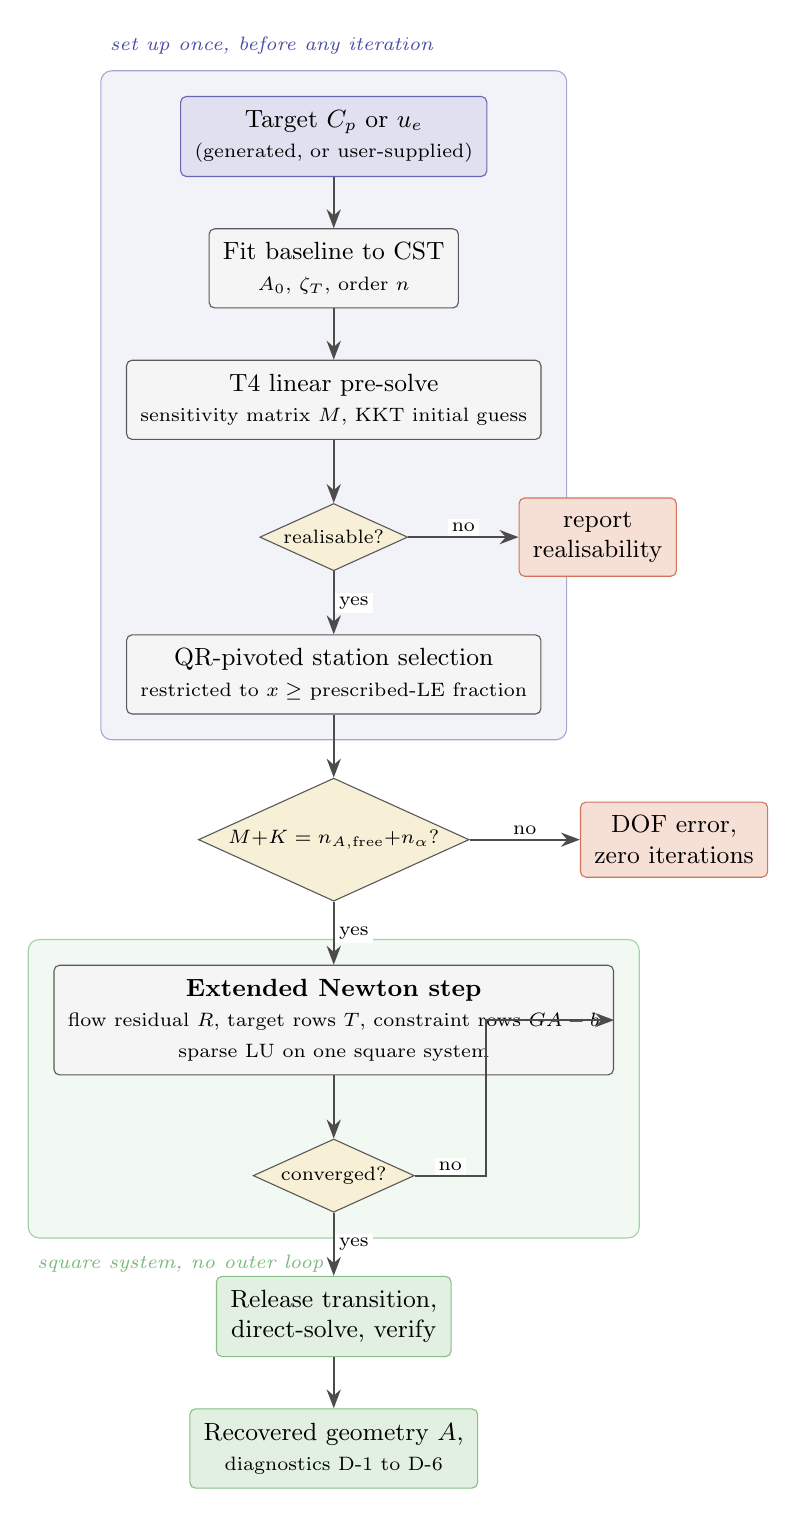
\begin{tikzpicture}[node distance=6.5mm and 9mm]
  \node[fcstart] (tgt) {Target $C_p$ or $u_e$\\ \scriptsize (generated, or user-supplied)};
  \node[fcbox, below=of tgt] (fit) {Fit baseline to CST\\ \scriptsize $A_0$, $\zeta_T$, order $n$};
  \node[fcbox, below=of fit] (pre) {T4 linear pre-solve\\ \scriptsize sensitivity matrix $M$, KKT initial guess};
  \node[fcdec, below=8mm of pre] (real) {realisable?};
  \node[fcfail, right=14mm of real] (warn) {report\\ realisability};
  \node[fcbox, below=8mm of real] (qr) {QR-pivoted station selection\\ \scriptsize restricted to $x \geq$ prescribed-LE fraction};
  \node[fcdec, below=8mm of qr] (sq) {$M{+}K = n_{A,\mathrm{free}}{+}n_\alpha$?};
  \node[fcfail, right=14mm of sq] (dof) {DOF error,\\ zero iterations};

  \node[fcbox, below=8mm of sq] (newt) {\textbf{Extended Newton step}\\
        \scriptsize flow residual $R$, target rows $T$, constraint rows $GA-b$\\
        \scriptsize sparse LU on one square system};
  \node[fcdec, below=8mm of newt] (conv) {converged?};
  \node[fcout, below=8mm of conv] (rel) {Release transition,\\ direct-solve, verify};
  \node[fcout, below=of rel] (out) {Recovered geometry $A$,\\ \scriptsize diagnostics D-1 to D-6};

  \begin{scope}[on background layer]
    \node[fit=(tgt)(qr), draw=NavyBlue!35, fill=NavyBlue!5, rounded corners,
          inner sep=3.2mm] (setup) {};
    \node[fit=(newt)(conv), draw=ForestGreen!40, fill=ForestGreen!6,
          rounded corners, inner sep=3.2mm] (loop) {};
  \end{scope}
  \node[anchor=south west, font=\scriptsize\itshape, NavyBlue!70]
        at ([yshift=0.8mm]setup.north west) {set up once, before any iteration};
  \node[anchor=north west, font=\scriptsize\itshape, ForestGreen!60]
        at ([yshift=-0.8mm]loop.south west) {square system, no outer loop};

  \draw[fcarrow] (tgt) -- (fit);
  \draw[fcarrow] (fit) -- (pre);
  \draw[fcarrow] (pre) -- (real);
  \draw[fcarrow] (real) -- node[fclab,above] {no} (warn);
  \draw[fcarrow] (real) -- node[fclab,right] {yes} (qr);
  \draw[fcarrow] (qr) -- (sq);
  \draw[fcarrow] (sq) -- node[fclab,above] {no} (dof);
  \draw[fcarrow] (sq) -- node[fclab,right] {yes} (newt);
  \draw[fcarrow] (newt) -- (conv);
  \draw[fcarrow] (conv) -- node[fclab,right] {yes} (rel);
  \draw[fcarrow] (rel) -- (out);
  \draw[fcarrow] (conv.east) -- ++(9mm,0) node[fclab,midway,above] {no}
        |- (newt.east);
\end{tikzpicture}
\caption{The monolithic inverse-design procedure. The pre-solve, station
selection and degree-of-freedom check all happen once, before any Newton
iteration; the loop then solves one square system per step with no outer
optimiser. The realisability gate reports rather than blocks, because
realisability is an inviscid-consistent quantity (\S\ref{sec:presolve}) and a
viscous target can be reachable while failing it. Algorithms~\ref{alg:monolithic}
and~\ref{alg:qrpivot} state the two shaded stages precisely.}
\label{fig:pipeline}
\end{figure}

Algorithm~\ref{alg:monolithic} states the full monolithic iteration, target
generation through release-and-verify, as pseudocode, making explicit where
each of \S\ref{sec:newton-system}--\S\ref{sec:presolve}'s mechanisms (FD
Jacobian assembly, joint under-relaxation, the trust region on $\Delta A$,
the forced-transition shim) sits inside the loop. It is a direct pseudocode
rendering of
\pth{src/cins/solver/newton.py::solve_inverse} and
\pth{src/cins/benchmarks/pipeline.py::run_pipeline}, not an idealisation
of it. Algorithm~\ref{alg:qrpivot} states the QR-pivoted station-selection
procedure identified as the identifiability guard in
\S\ref{sec:ablations} (\pth{src/cins/benchmarks/pipeline.py}, station-
selection step), reusing the T4 pre-solve sensitivity matrix rather than
building a second one.

\begin{algorithm}
\caption{Monolithic CST--Newton inverse iteration (\S\ref{sec:newton-system}--\S\ref{sec:presolve})}
\label{alg:monolithic}
\begin{algorithmic}[1]
\Require target airfoil (for $A^\ast$ generation) or externally supplied $Cp_{target}$; Bernstein order $n$; \texttt{le\_treatment}; \texttt{transition.mode}
\State Fit CST to reference geometry $\rightarrow A^\ast$ (\S\ref{sec:cst-linearity}); build $\partial\zeta/\partial A_i = C(\psi)S_i(\psi)$ once, cache (Eq.~\eqref{eq:dsurface-dA})
\State Generate target: direct-solve at $A^\ast$ (forced transition if \texttt{mode=forced}, \S\ref{sec:transition}) $\rightarrow Cp_{target}^{\text{full}}$
\State Perturb or randomize $A^\ast \rightarrow A_0$ (T8 \texttt{init} factor); assemble $G,b$ from \S\ref{sec:constraints}
\If{\texttt{init = presolve}}
  \For{2 passes} \Comment{T4 pre-solve, \S\ref{sec:presolve}}
    \State Build sensitivity matrix $M$ at current $A_0$ (finite-difference or Beta-function analytic)
    \State Solve KKT system Eq.~\eqref{eq:kkt} for $A_0$; record realisability, model\_gap (ADR-0004, two \emph{distinct} metrics)
  \EndFor
\EndIf
\State Select $M$ target stations by QR pivoting (Algorithm~\ref{alg:qrpivot}) or evenly-spaced (T8 ablation)
\State \textbf{Assert} $M+K=n_{A,\text{free}}+n_\alpha$ (Eq.~\eqref{eq:dof}, FM-1 guard) \Comment{raises before any Newton step if violated}
\State Direct-solve flow at $A_0$ (converges $U_0$) \Comment{initial point for the extended Newton loop}
\State $k \gets 0$
\While{$\|R\|,\|T\|,\|G\| >$ \texttt{rtol} and $k <$ \texttt{max\_iter}} \Comment{D-1 per-block residual norms}
  \State Assemble $\partial R/\partial U$, $\partial R/\partial\alpha$ from mfoil (analytic, unchanged)
  \State Assemble $\partial R/\partial A$ by central finite differences over $A$ only (\S\ref{sec:derivatives}), $O(n_A)$ residual evaluations
  \State Assemble $\partial T/\partial U$ (Cp-selection map), $\partial G/\partial A = G$ (constant)
  \State Solve linearised system $J\,\delta \gets -[R;T-Cp_{target};G\cdot A-b]$ (Eq.~\eqref{eq:jacobian-blocks})
  \State Compute joint under-relaxation $\omega\in(0,1]$: the smaller of mfoil's own $U$-limiter (Hk, $\theta$/$\delta^*$ bounds) and the CST trust region $\|\delta_A\|_\infty \leq$ \texttt{a\_trust\_radius} (\S\ref{sec:newton-system})
  \State $U \gets U + \omega\,\delta_U$; $A \gets A + \omega\,\delta_A$; $\alpha \gets \alpha + \omega\,\delta_\alpha$ (if free)
  \State Rebuild geometry from updated $A$ (apply\_geometry, \S\ref{sec:cst-linearity}); record D-2..D-6 diagnostics
  \State $k \gets k+1$
\EndWhile
\State \textbf{Release-and-verify} (\S\ref{sec:transition}): un-force transition; direct-solve at converged $A$; assert $\Delta c_l, \Delta c_d$ against the natural-mode target within gate
\State \Return $A$, iteration count $k$, residual history, release-and-verify record
\end{algorithmic}
\end{algorithm}

\begin{algorithm}
\caption{QR-pivoted target-station selection (\S\ref{sec:ablations})}
\label{alg:qrpivot}
\begin{algorithmic}[1]
\Require sensitivity matrix $M\in\mathbb{R}^{N_{cand}\times n_A}$ from the T4 pre-solve (\S\ref{sec:presolve}); free-coefficient index set $\mathcal{F}$; required station count $M_{req} = n_{A,\text{free}} - K + n_\alpha$
\State Restrict candidates to nodes at or aft of the prescribed-LE fraction (FM-3 mitigation, \S\ref{sec:fm})
\State Form the candidate submap $\tilde M \gets M[\text{candidates},\, \mathcal{F}]$
\State Column-pivoted QR: $\tilde M^\top P = QR$, giving a pivot ordering $P$ by decreasing contribution to $\tilde M^\top$'s numerical rank
\State Select the first $M_{req}$ pivoted candidate indices $\rightarrow$ target stations
\State \Return sorted station index set; report $\mathrm{cond}(\tilde M[\text{stations},:])$ (D-3-class diagnostic, \emph{distinct} from $\mathrm{cond}(J)$, ADR-0004)
\end{algorithmic}
\end{algorithm}

\subsection{Forced-transition onset closure}
\label{sec:transition}
% <- ADR-0003 (revised mechanism); FM-4, mfoil's (and XFOIL's) $e^n$ transition closure is only $C^0$ in the design
variables: the transition-station equation itself performs an internal
sub-Newton solve for the point $x_t$ where the marched amplification factor
crosses $n_{crit}$, and that location moves discontinuously as geometry
changes cross a threshold. A coupled Newton iteration needs a continuous
residual; a kink stalls or chatters it (dossier~\S4, FM-4). The mitigation
prescribed by the dossier is to fix (trip) transition during the inverse
iterations and release it for a verification solve afterward. mfoil exposes
no forced-trip API, so this is implemented as an adapter-level shim
(ADR-0003) rather than a vendor-code edit.

The first implementation attempt froze the laminar/turbulent node flags
(\texttt{M.vsol.turb}) and no-op'd mfoil's own \texttt{update\_transition},
but left the natural \texttt{residual\_transition} equation untouched at the
frozen boundary station. This was \emph{insufficient}. Empirically (NACA
2412, $\alpha=2^\circ$, $Re=10^6$, trip 5\%/5\%), the physics moved correctly
under Newton pressure ($c_d$: 0.00578 $\to$ 0.00741), but the solve never
converged. \texttt{Rnorm} stalled at $\approx12.6$ for the full 50-iteration
budget, because the frozen station equation still solves internally for
amplification $= n_{crit}$, which has no solution once transition is pinned
somewhere amplification is nowhere near $n_{crit}$ (ADR-0003, ``Revision'').
The corrected mechanism, \texttt{\_residual\_transition\_forced}, replaces
the boundary-station residual with an XFOIL-style turbulence-\emph{onset}
closure: the momentum and shape-parameter rows use the ordinary turbulent
\texttt{residual\_station} closure directly across the whole station (no
laminar sub-leg, no station-local $x_t$), and the shear-lag row is replaced
with the same onset condition mfoil's own \texttt{update\_transition} uses to
initialize a newly-turbulent node, $U_2[2] = c_{ttr}(U_2)$, which depends
only on the downstream state (ADR-0003). With this closure, the shim
converges cleanly: trip 5\%/5\% reaches \texttt{glob.conv=True},
$\mathrm{Rnorm}<10^{-10}$, $c_d=0.01125$ (strictly $>$ natural
$c_d=0.005778$, as physically expected for larger turbulent wetted area).
Trip 30\%/30\% gives $c_d=0.00788$, strictly between the 5\%-trip and natural
values, monotonic in trip location. Releasing transition and re-solving
from the converged forced state reproduces the pinned natural baseline to
within its stated tolerance ($c_l=0.449351\pm10^{-3}$,
$c_d=0.005778\pm2\times10^{-4}$). These figures are from the shim's own
verification run (ADR-0003) and differ in the fourth decimal from the T7
archive's release-and-verify values quoted in \S\ref{sec:falsifiable}
($c_l=0.449091$, $c_d=0.005774$), which is a different run at a different
paneling, not a restatement of the same one. Rebuilding the global system after
convergence with the shim still active reproduces $\|R\|<10^{-8}$: the
converged state is a genuine fixed point of the forced residual, not an
artifact of the step sequence (ADR-0003, ``Consequences''). Every T7/T8
result reported in \S\ref{sec:results} therefore states its transition mode
explicitly, and release-and-verify in natural-transition direct mode is part
of the T7 protocol (\S\ref{sec:falsifiable}), not an optional extra.

Figure~\ref{fig:viscous} shows the state this closure operates on, and is
the reason a coupled solver was required rather than an inviscid one with a
boundary-layer post-process. The inverse system of
\S\ref{sec:newton-system} is appended to mfoil's \emph{viscous} global
system, so the six distributions in the figure are unknowns inside the same
Newton solve that recovers the geometry, not quantities computed afterwards
from a converged pressure field. Panel~(f) makes the coupling explicit: the
displacement thickness $\delta^*$ displaces the effective body the inviscid
half sees, and it is through that term that a geometry perturbation reaches
the boundary layer and back. The trip locations are marked on each panel;
the skin-friction rise at the trip in panel~(c) and the corresponding drop
in shape factor in panel~(d) are the closure described above taking effect.

\begin{figure}[htbp]
\centering

\includegraphics[width=\textwidth]{fig_viscous_solution.png}
\caption{The coupled viscous solution the inverse system is embedded in,
for NACA 2412 at $\alpha=2^\circ$, $\Rey=10^6$, with transition forced at 5
percent chord on both surfaces (dotted lines).
(a)--(b)~momentum and displacement thickness; (c)~skin friction, rising at
the trip; (d)~kinematic shape factor; (e)~edge velocity, the quantity the
inviscid half exchanges with the boundary layer; (f)~the displacement
surface $\zeta\pm\delta^*$, which is the coupling term itself. All six are
state variables of the same global system to which the CST coefficients are
appended.}
\label{fig:viscous}
\end{figure}

\subsection{Analytic pre-solve and realisability}
\label{sec:presolve}
% <- T4; ADR-0004 realisability semantics

Two jobs are done by a single linear pre-solve before any Newton iteration
runs, and the distinction between them is load-bearing for how results are
reported (ADR-0004). Thin-airfoil theory is linear in camber slope and
thickness, and CST camber/thickness are linear in $A$, so
$Cp_{target}\approx M\cdot A$ for a sensitivity matrix $M$ built either
analytically (the Joseph--Mohan Beta-function kernels) or, as implemented,
numerically from mfoil's own linear-vorticity panel influence coefficients
at fixed geometry. Solving the constrained least-squares problem with the
\S\ref{sec:constraints} rows as linear equality constraints,
\begin{equation}
  \begin{bmatrix} M^\top M & G^\top \\ G & 0 \end{bmatrix}
  \begin{bmatrix} A \\ \lambda \end{bmatrix}
  = \begin{bmatrix} M^\top Cp_{target} \\ b \end{bmatrix},
  \label{eq:kkt}
\end{equation}
gives (1) an initial guess placing Newton inside its basin
of attraction: the LE region is exactly where Newton wanders, and mfoil's
own documentation warns the coupled solver can fail from a poor initial
guess; and (2) a \textbf{realisability} metric,
$\|M A^\ast - Cp_{target}\|/\|Cp_{target}\|$, that flags targets outside the
CST-representable manifold \emph{before} a Newton solve is attempted.

An adversarial T4/T5/T7 review found these two jobs' outputs had been
conflated into one number, and ADR-0004 is the resulting decision, binding
for every number reported in this paper:

\begin{quote}
1.\ \textbf{CST-representability} (the realisability guard, above) must be
answered with \emph{model-consistent} quantities: inviscid target against
inviscid linearisation. On the T7 winning configuration this is
$3.90\times10^{-4}$; the target is
representable. 2.\ \textbf{Model gap}, how far the inviscid linearisation
sits from the viscous physics the Newton solve actually faces, is a
\emph{separate}, diagnostic-only quantity, $0.110$ on the same case. This is boundary-layer displacement
effect, which no inviscid model captures. It is \emph{not} target
unrealisability; the subsequent monolithic solve converging to
$2.75\times10^{-11}$ (\S\ref{sec:falsifiable}) is direct proof the target
was realisable despite the nonzero model gap.
\end{quote}

\textbf{Reporting rule, enforced throughout this paper:} realisability
numbers are always labelled with their model (``inviscid-consistent''), and
the conditioning of the QR-selected station submap ($\mathrm{cond}\approx90$,
\S\ref{sec:ablations}) is never quoted as the conditioning of the full
extended Newton system. These are different
matrices answering different questions; conflating them was one of the
review's confirmed findings.


% =====================================================================
\section{Failure modes and their instrumentation}
\label{sec:fm}
\label{sec:fm}
% FM-1 rank/DOF, FM-2 Bernstein conditioning, FM-3 LE-singular rows, FM-4 C0
% viscous closure; diagnostics D-1..D-6.                % <- T6, SPEC.md \S6

Four failure modes were identified a priori
(\dossierref{\S4}) as the ways the
architecture of \S\ref{sec:formulation} can fail without that failure being
obviously attributable to its true cause. Table~\ref{tab:fm} summarises
each, its diagnostic, and its mitigation; \S\ref{sec:newton-system}--
\S\ref{sec:presolve} describe FM-1, FM-4's mechanism and FM-1's realisability
guard in detail, and \S\ref{sec:ablations} reports the empirical FM-2 cliff.

\begin{table}[h]
\centering
\caption{The four failure modes identified a priori, each with the
diagnostic that detects it and the mitigation adopted. All four were
predicted before implementation and all four were observed; the instrumentation
exists so that a failed solve reports which mode it hit rather than only that
it failed. Source: SPEC.md~\S8, \dossierref{\S4}.}
\label{tab:fm}
\footnotesize
\begin{tabularx}{\textwidth}{@{}l l L L L@{}}
\toprule
ID & Name & Mechanism & Diagnostic & Mitigation \\
\midrule
FM-1 & DOF/realisability & rank-deficient or over-determined & D-2 (rank/cond $J$) & Eq.~\eqref{eq:dof} assertion; T4 realisability \\
FM-2 & Bernstein conditioning & Gram matrix $\mathrm{cond}\sim4^n$ & D-3 ($\mathrm{cond}(G^\top G)$ vs $n$) & keep $n\lesssim10$--12/side; orthogonalise \\
FM-3 & LE-singular Jacobian rows & $\sqrt\psi$ non-analytic at $\psi=0$ & D-4 (row-norm vs station) & row scaling; prescribed-LE (\S\ref{sec:falsifiable}) \\
FM-4 & $C^0$ viscous closure & transition-station kink & D-5 (transition history) & forced trip, release-and-verify (\S\ref{sec:transition}) \\
\bottomrule
\end{tabularx}
\end{table}

The remaining diagnostics, D-1 (per-block residual norms, discriminates
\emph{which} block stalls) and D-6 (Newton convergence history, the
headline figure confirming the quadratic-tail architectural claim), are
not tied to a single failure mode; they are the general-purpose instruments
used throughout \S\ref{sec:results}. FM-3's fix targets
\emph{rows}, not columns: \S\ref{sec:cst-linearity} showed
$\partial\zeta/\partial A_i$ is perfectly finite as $\psi\to0$ (it tends to
zero), so the geometric columns are healthy. What blows up is the flow
residual's \emph{sensitivity} to geometry near the nose (surface normals,
metric terms, the stagnation-point mapping all have unbounded derivatives
there), so a handful of rows near the stagnation point acquire enormous
magnitude and destroy the coupled matrix's condition number. This is a
concrete instance of the point made in
\S\ref{sec:cst-linearity}: CST's linearity keeps the columns exact, but does
not by itself guarantee the rows are well-conditioned near a genuinely
non-analytic geometric feature.


% =====================================================================
\section{The falsifiable test}
\label{sec:falsifiable}
The architecture's central claim, that appending CST coefficients to
\texttt{mfoil}'s Newton system yields a determined root-find rather than a
search, is falsifiable by a single self-consistency experiment with a
\emph{known} answer, guaranteed realisable by construction. The protocol fits
CST to a known airfoil, runs \texttt{mfoil} in direct mode to generate a
target pressure and edge-velocity distribution from that fit, perturbs the
coefficients or uses the pre-solve of Section~\ref{sec:presolve} to obtain a
starting guess, and asks whether the monolithic inverse Newton iteration
recovers the original coefficient vector $A^\ast$, following the procedure
stated as pseudocode in Section~\ref{sec:algorithms}. Any failure of this test
isolates cleanly to one of the Table~\ref{tab:fm} failure modes rather than to
target infeasibility. This is why this test, and not a search over
independently chosen targets, is the load-bearing evidence for the hypothesis.
It is also, by the same construction, the test's principal weakness, and
Section~\ref{sec:validity} states that weakness in full rather than leaving it
implicit here.

\paragraph{Reference configuration.} NACA 2412, $n=8$ per side, leading edge
prescribed, meaning the first 5 percent of chord is fixed geometrically rather
than left inverse. That is the mixed direct-inverse mitigation for the
leading-edge failure mode of Section~\ref{sec:fm}, and it is the cheapest test
of the whole hypothesis because it isolates the leading-edge question from the
architecture question. Transition is forced during the inverse iterations
(Section~\ref{sec:transition}), target stations are chosen by QR column
pivoting (Section~\ref{sec:ablations}), the iteration is initialised from the
linear pre-solve, and the angle of attack is held fixed. This configuration is
referred to throughout the rest of the paper as the reference configuration.

\paragraph{Protocol, including release-and-verify.} The success criterion is
$\norm{A-A^\ast}_\infty < 10^{-4}$ within nine Newton iterations, together with
a residual history showing sustained superlinear decrease. Because the inverse
solve runs under the forced-transition closure of
Section~\ref{sec:transition}, the protocol additionally requires releasing
transition and re-solving in fully natural, direct mode at the recovered
geometry, then comparing the resulting aerodynamic coefficients against those
of the \emph{reference section} solved in the same natural mode. This is a
check that the forced-transition inverse solve recovered the geometry, rather
than merely finding a zero of the forced-mode residual that happens to be
aerodynamically different.

\paragraph{Result.} Measured against the $10^{-4}$ and nine-iteration
criterion, the solve returns $\norm{A-A^\ast}_\infty = 2.747\x10^{-11}$ in six
Newton iterations, with the target-block residual history
$5.85\x10^{-4} \to 2.05\x10^{-5} \to 1.57\x10^{-7} \to 1.21\x10^{-8} \to
2.13\x10^{-10} \to 9.47\x10^{-12}$, plotted alongside the ablation runs in
Figure~\ref{fig:convergence}. Release-and-verify against a
$\Delta c_l<10^{-3}$, $\Delta c_d<2\x10^{-4}$ criterion gives
$\Delta c_l = 3.4\x10^{-12}$ and $\Delta c_d = 3.0\x10^{-14}$, both essentially
at floating-point noise: the released solve at the recovered geometry
reproduces the reference section's natural-transition coefficients
($c_l=0.449091$, $c_d=0.005774$) to machine precision. Because both sides of
that comparison are natural-mode solves at geometries agreeing to
$2.7\x10^{-11}$, agreement at this level is what smoothness alone would
predict; the check confirms that no aerodynamically distinct root was reached,
and should not be read as independent evidence of accuracy. Realisability,
computed inviscid-consistently as Section~\ref{sec:presolve} requires, is
$3.90\x10^{-4}$; the model gap, diagnostic only, is $0.110$. Sixteen
coefficients are \emph{recovered} by the Newton iteration; the two
leading-edge coefficients $A_{u,0}$ and $A_{l,0}$ are \emph{prescribed} by the
configuration and are not recovered, so all error norms quoted here are over
the 16 free coefficients. Table~\ref{tab:t7} collects the criteria and the
measured values.

\begin{table}[htbp]
\centering
\caption{The falsifiable test at the reference configuration: every criterion
met, each by several orders of magnitude.}
\label{tab:t7}
\begin{tabularx}{\textwidth}{@{}L c c@{}}
\toprule
Criterion & Threshold & Measured \\
\midrule
$\norm{A-A^\ast}_\infty$ over the 16 free coefficients & $<10^{-4}$ & $2.747\x10^{-11}$ \\
Newton iterations & $\leq9$ & $6$ \\
Sustained decrease of the target block & required & 7 decades over 5 steps \\
Release-and-verify $\Delta c_l$ & $<10^{-3}$ & $3.4\x10^{-12}$ \\
Release-and-verify $\Delta c_d$ & $<2\x10^{-4}$ & $3.0\x10^{-14}$ \\
\bottomrule
\end{tabularx}
\end{table}

An independently-run six-vector adversarial review probed circularity,
station-index correspondence, the pinned-coefficient framing, the absence at
the time of a release-and-verify step, realisability semantics, and the
conflation of submap conditioning with system conditioning. Every confirmed
finding is reflected in this paper's reporting discipline: the split between
free and prescribed coefficients above, and the two-metric realisability rule
of Section~\ref{sec:presolve}. The station-index correspondence finding was
closed differently from the others. It was originally answered with a numeric
guard, asserting that the selection-time node and the target's own paneling
agreed to $\max|\Delta x/c|<2\x10^{-5}$. That guard has since been removed,
because addressing a station by surface and chordwise fraction, and
interpolating the target's own pressure curve at that fraction, makes the
correspondence exact rather than approximate, so there is no longer a quantity
for the guard to bound. Two consequences are recorded here rather than left
implicit. Interpolated addressing is what introduces the neglected
$\partial T/\partial A$ term of Section~\ref{sec:newton-system}, and with it
the inexact-Newton behaviour analysed in Section~\ref{sec:h3}. And the runs of
Section~\ref{sec:results}, which predate the change, retain the earlier
nearest-node addressing with a residual correspondence error of up to
$2.0\x10^{-4}$ in chord fraction, ten times the bound the retired guard
imposed; Section~\ref{sec:results} states where that matters.

\begin{figure}[htbp]
\centering

\includegraphics[width=0.75\textwidth]{h3_convergence_overlay.png}
\caption{Newton residual history of the node-indexed baseline run, overlaid
with the evenly-spaced-station wrong-root case and the $n=12$
conditioning-cliff case of Section~\ref{sec:ablations}.}
\label{fig:convergence-overlay}
\end{figure}

Figure~\ref{fig:convergence-overlay} places that history in context by
overlaying the node-indexed baseline against the two ablation runs that fail
for different reasons, the evenly-spaced-station case that converges to a
wrong root and the $n=12$ case that converges slowly; all three are analysed
in Section~\ref{sec:ablations}. A residual history is in any case a scalar
summary. Figures~\ref{fig:t7-geometry} to~\ref{fig:t7-flow} give the geometry
and flow-field view of the same result, regenerated directly from a fresh
re-run of the reference configuration rather than hand-plotted.
Figure~\ref{fig:t7-geometry} overlays the target and Newton-recovered airfoil
outlines, visually indistinguishable at full-chord scale, with a leading-edge
inset showing the same at the scale where the leading-edge failure mode would
be visible if the prescribed-nose mitigation were absent. It also includes a
per-coefficient recovery-error bar chart making explicit which two of eighteen
coefficients are pinned rather than recovered.

\begin{figure}[htbp]
\centering

\includegraphics[width=0.85\textwidth]{paper/fig_t7_geometry_overlay.png}
\caption{Target against Newton-recovered geometry at the reference
configuration, with a leading-edge inset and a per-coefficient recovery-error
bar chart. Grey bars are prescribed, not recovered.}
\label{fig:t7-geometry}
\end{figure}

Figure~\ref{fig:t7-cp} compares target and recovered pressure distributions
both as a full curve and restricted to the 16 QR-pivoted stations the Newton
system actually solved against. The distinction matters: agreement at the
solved stations is enforced by construction, whereas agreement away from them
is not, and it is the full curve that shows the recovered geometry reproduces
the target everywhere rather than only where it was sampled. This is the
pressure-level counterpart of the coefficient-level agreement in
Table~\ref{tab:t7}, and rules out the possibility that the reported error is
an artifact of comparing only at the fitted stations.

\begin{figure}[htbp]
\centering

\includegraphics[width=0.95\textwidth]{paper/fig_t7_cp_comparison.png}
\caption{Target against recovered pressure distribution under forced
transition, plotted in the aerodynamic convention with inverted vertical axis:
full curve (left) and the 16 QR-pivoted target stations only (right).}
\label{fig:t7-cp}
\end{figure}

Figure~\ref{fig:t7-flow} shows the converged, released, natural-transition
flow solution at the recovered geometry: the pressure distribution and the
boundary-layer displacement thickness. This is the physical state from which
the release-and-verify comparison of Table~\ref{tab:t7} was computed, and the
displacement-thickness panel is worth reading alongside
Figure~\ref{fig:viscous}: with transition released, the laminar run extends
well aft of the 5 percent trip used during the inverse iterations, which is
precisely the difference the release step exists to check the solve did not
absorb into geometry.

\begin{figure}[htbp]
\centering

\includegraphics[width=0.95\textwidth]{paper/fig_t7_flow_solution.png}
\caption{Converged flow solution at the recovered geometry after transition is
released: pressure distribution (left) and displacement thickness
$\delta^*/c$ (right).}
\label{fig:t7-flow}
\end{figure}


% =====================================================================
\section{Ablations and results}
\label{sec:results}
\label{sec:results}
% <- T8; ablations from paper/results_digest.md; identifiability LEADS.
% CAVEAT (state once, applies to every subsection): all T8 numbers are N=1
% (single seed=42 run per cell); no confidence intervals are statistically
% defensible at N=1 (STATS_PROTOCOL Stage-1-lite scoping). T8 as executed is
% a single-airfoil (NACA 2412) ablation matrix plus two extra single-airfoil
% cells (0012, 4415), NOT the pre-registered ~20-section NACA panel
% (configs/experiments/panel_naca.yaml does not exist). Source:
% paper/results_digest.md preamble; experiments/results/t8/ANALYSIS.md \S0.

Every number in this section traces to a \texttt{result.json} or
\texttt{diagnostics.json} artifact under \pth{experiments/results/t8/}
(paper/results\_digest.md; per-cell citation in
\pth{experiments/results/t8/ANALYSIS.md}). All values are $N{=}1$
(single \texttt{seed=42} run per cell); no confidence intervals are reported
because none are statistically defensible at $N{=}1$, per
\pth{docs/STATS_PROTOCOL.md}'s Stage-1-lite scoping. The $n$-sweep,
station-selection, and other single-factor \emph{ablation} tables in this
section are a single-airfoil (NACA 2412) matrix plus two extra
single-airfoil cells (0012, 4415). These are deliberately narrow,
$N{=}1$-per-cell comparisons designed to isolate one factor at a time, not
a panel study.
Panel-level convergence-\emph{fraction} language is deliberately avoided in
those subsections for that reason. \S\ref{sec:h1-panel} is the one
exception: it reports the pre-registered $\approx$20-section NACA panel
(\pth{configs/experiments/panel_naca/*.yaml}), run subsequently at the
winning configuration identified by this section's ablations, and its
Wilson-interval convergence-fraction claim is reported there on its own
terms.

\paragraph{Station-addressing provenance.} The ablation matrix in this
section was run with target stations addressed by panel-node index, which was
the implementation at the time. Addressing was subsequently changed to
$(\text{surface}, x/c)$ with interpolation between the two bracketing nodes,
because a node index stops denoting the same physical location once the
geometry moves, which is precisely what an inverse solve does
(\S\ref{sec:newton-system}). The change moves the T7 figures quoted in
\S\ref{sec:falsifiable} from $1.08\times10^{-11}$ in 4 iterations to
$2.75\times10^{-11}$ in 6, both far inside the $10^{-4}$/9-iteration gate,
and leaves the QR-selected submap conditioning unchanged at 90.3. Every cell
in this section shares the earlier addressing, so the within-matrix
comparisons that the ablations rest on are unaffected; what must not be done
is to read a single number from this section alongside a single number from
\S\ref{sec:falsifiable} as though they came from one run. Where that
distinction matters, it is stated at the point of use.

\subsection{Station-selection identifiability: the central methodological result}
\label{sec:ablations}

This finding leads the ablation discussion, ahead of the flow-solve count,
because it is the most novel, most precisely quantified, and most
consequential result in T8 (benchmarks/REPORT.md, ``Recommendations for
P1''). The square extended Newton system (\S\ref{sec:newton-system}) demands
exactly $M$ target-station equations. With evenly-spaced stations, between-
station Cp information is discarded, and the resulting $16\times16$ station-
sensitivity submap can be badly ill-conditioned. Table~\ref{tab:identifiability}
reports the two configurations that isolate this mechanism.

\begin{table}[h]
\centering
\caption{Station-selection ablation, the paper's central methodological
result. Both cells report \texttt{converged: true} and drive the residual to
the solver floor, yet their recovery errors differ by eight orders of
magnitude: only the QR-pivoted selection recovers the generating design, and
the evenly-spaced selection converges to a spurious root while its station
submap conditions at $3\times10^{12}$. Source:
\pth{experiments/results/t8/ANALYSIS.md}~\S4.}
\label{tab:identifiability}
\begin{tabular}{lccc}
\toprule
Selection & $\mathrm{err\_all\_inf}$ & Submap $\mathrm{cond}$ & Newton \texttt{converged} flag \\
\midrule
\texttt{qr\_pivot} (winning config) & $\mathbf{1.08\times10^{-11}}$ & 90.3 & \texttt{true} \\
\texttt{even} (evenly-spaced) & $\mathbf{1.43\times10^{-3}}$ (FAILS $10^{-4}$ gate) & $3.47\times10^{12}$ & \texttt{true} \\
\bottomrule
\end{tabular}
\end{table}

Both cells' Newton loops report their own internal \texttt{converged: true};
the residual reaches the solver's floor in both cases. \textbf{Only
\texttt{qr\_pivot} recovers the correct design.} ``Converged'' and
``correct'' are different claims, invisible unless $\mathrm{err\_all\_inf}$
is checked against the true coefficients rather than the residual norm
alone (experiments/results/t8/ANALYSIS.md~\S0, Deviation 5). The mechanism:
with evenly-spaced stations, near-null coefficient directions exist whose
motion changes the sampled Cp by less than floating-point precision.
Newton converges to \emph{any} of several exact roots of the (badly-
conditioned) discrete system, a structural non-uniqueness of the sampled
problem, not a numerical accident. This reproduces and sharpens a pre-T8
finding (\pth{docs/triz/T7-identifiability.md}: cond $\sim10^7$, error
$1.4\times10^{-3}$--$6\times10^{-2}$ with evenly-spaced stations) with a
controlled ablation cell. Two contributing null-direction families were
identified and eliminated \emph{before} the station-selection fix, each
verified empirically (\pth{docs/triz/T7-identifiability.md}): a
camber--$\alpha$ equivalence (freeing $\alpha$ lets a slightly different
camber at a slightly different $\alpha$ interpolate the same samples, so
$\alpha$ is fixed for self-consistency tests), and a prescribed-LE mismatch
(excluding LE stations while leaving the LE-dominant coefficients free
leaves $A_0$ unobservable, which is why \texttt{le\_treatment=prescribed}
\emph{fixes} $A_{u,0}$/$A_{l,0}$ rather than merely dropping LE-region
target rows).

The resolution keeps the system square, with no least-squares relaxation
and no reintroduced optimisation, and instead makes each of the $M$
equations maximally informative. The T4 pre-solve (\S\ref{sec:presolve})
already builds the full $(200\times n_A)$ sensitivity matrix for
initialisation; reusing it to \emph{select} the $M$ target stations by QR
column pivoting chooses the rows that maximise the resulting square
submap's conditioning. The measured effect: submap condition
$10^7\to90.3$; recovery error $1.4\times10^{-3}\to1.08\times10^{-11}$.
Full-curve sensitivity information enters only through the
(already-required) linear pre-solve, and the nonlinear Newton solve stays
square and determined throughout (\pth{docs/triz/T7-identifiability.md}).
Sensitivity-optimal station selection is therefore the identifiability
guard for determined inverse systems, a methodological contribution of this
paper beyond the original dossier hypothesis: a practical answer to the
non-uniqueness caveat inverse problems inherit from Lighthill's and
Volpe \& Melnik's well-posedness constraints
(\S\ref{sec:presolve}; \dossierref{\S7.10}),
without abandoning the root-finding architecture for a least-squares
relaxation.

Figure~\ref{fig:station-selection} summarises the ablation of
Table~\ref{tab:identifiability}: the same solver, the same target and the
same convergence flag produce recovery errors eight orders of magnitude
apart, separated only by which stations were sampled.

\begin{figure}[h]
\centering

\includegraphics[width=0.75\textwidth]{station_selection.png}
\caption{Station-selection identifiability at a glance: recovery error, QR-pivoted vs.\ evenly-spaced target stations, annotated with submap conditioning. Source: \pth{experiments/results/t8/figures/station_selection.png}.}
\label{fig:station-selection}
\end{figure}

\subsection{Where the stations are placed: the prescribed leading edge}
\label{sec:le-identifiability}

\S\ref{sec:ablations} records one half of a requirement: excluding
leading-edge target stations while leaving the LE-dominant coefficients free
leaves $A_0$ unobservable, which is why \texttt{le\_treatment=prescribed}
fixes $A_{u,0}$ and $A_{l,0}$ rather than merely dropping LE-region rows. The
other half is the converse, and it was found while extending the method to
arbitrary user-supplied targets: once the leading edge \emph{is} prescribed,
the LE-region target stations must in turn be excluded. The two conditions are
not independent choices. Prescribing the nose without restricting the
candidate stations, or restricting the stations without prescribing the nose,
each leaves a near-null direction in the sampled system; only the pair is
identifiable.

Under the prescribed-LE treatment (FM-3, \S\ref{sec:fm}), $A_{u,0}$ and
$A_{l,0}$ are given rather than solved, so a target row placed inside the
prescribed region constrains pressure over a piece of surface that cannot
move. The effect on sampling is not a uniform loss of information, and
Figure~\ref{fig:le-identifiability}(a) is worth reading carefully on this
point. Across the prescribed region the norm of
$\partial C_p/\partial A_{\text{free}}$ spans nearly two orders of magnitude,
from $0.054$ at the nose itself to $3.90$ just aft of it, against a median of
$1.47$ over the rest of the chord. The region therefore contains both the
single least informative station on the surface and some of the most
sensitive. That combination is what makes unrestricted QR selection a poor
choice here rather than merely a neutral one: the pivoting is drawn to the
high-sensitivity nose stations, and the rows it selects there are strongly
mutually correlated, because a small neighbourhood of a fixed nose produces
nearly the same pressure response for every free coefficient. The extended
system stays formally square and full-rank while becoming numerically
near-dependent, which is the same underlying condition as
Table~\ref{tab:identifiability} reached from the opposite direction.

Restricting the QR candidate set to $x \geq$ the prescribed-LE fraction, as
Algorithm~\ref{alg:qrpivot} specifies, removes the degeneracy.
Table~\ref{tab:le-identifiability} reports the effect on a self-consistency
target, holding everything else fixed.

\begin{table}[h]
\centering
\caption{Target-station placement under a prescribed leading edge. Both cells
start from the same perturbed geometry and differ only in whether the QR
candidate set is restricted to $x \geq$ the prescribed-LE fraction. With the
leading-edge region left in the candidate set the solve does not converge at
all within the 50-iteration budget, despite driving its residual to
$1.9\times10^{-10}$. Surface offset is quoted in millichords, against the 1
millichord that \S\ref{sec:formulation}'s fit gate allows a CST
representation itself. Source:
\pth{experiments/results/le_stations/result.json}.}
\label{tab:le-identifiability}
\footnotesize
\begin{tabularx}{\textwidth}{@{}L c c@{}}
\toprule
Quantity & LE stations in candidate set & LE stations excluded \\
\midrule
Candidate stations          & 200                   & 169 \\
Submap condition            & $31.7$                & $19.9$ \\
Converged                   & \textbf{no}           & \textbf{yes} \\
Newton iterations           & 50 (budget exhausted) & \textbf{7} \\
Final residual              & $1.89\times10^{-10}$  & $8.21\times10^{-11}$ \\
$\norm{A-A^*}_\infty$ (free)& $6.97\times10^{-1}$   & $\mathbf{4.10\times10^{-3}}$ \\
Max surface offset (mc)     & $11.74$               & $\mathbf{0.127}$ \\
\bottomrule
\end{tabularx}
\end{table}

The residual is not what separates the two columns. The unrestricted cell
drives its residual to $1.9\times10^{-10}$, within an order of magnitude of
the restricted cell's, and still fails to converge inside a 50-iteration
budget while ending $11.7$ millichords from the target surface. Restricting
the candidate set converges in 7 iterations to $0.127$ millichords, a
ninety-fold improvement in the recovered shape, with the submap conditioning
improving only from $31.7$ to $19.9$. A conditioning number that moves by
less than a factor of two therefore does not bound the effect: what matters
is whether the equations are spent on a part of the surface the solver is
allowed to move.

This reinforces rather than repeats \S\ref{sec:ablations}. There, the
degeneracy came from discarding between-station information across the whole
chord, and both configurations converged, one of them to a wrong root. Here
it comes from spending equations on a region that has been removed from the
design space, and the failure is visible as non-convergence rather than as a
confident wrong answer. Neither is detectable from the residual norm alone.

\begin{figure}[htbp]
\centering

\includegraphics[width=\textwidth]{fig_le_identifiability.png}
\caption{Why target stations must be kept out of a prescribed leading edge.
(a)~the sensitivity of surface pressure to the free coefficients across the
chord, with the prescribed region shaded: it does not vanish there but varies
by nearly two orders of magnitude, holding both the least and some of the most
sensitive stations; (b)~the stations chosen by unrestricted
QR against those chosen from the restricted candidate set, with the resulting
submap conditioning; (c)~the effect on the solve, plotted relative to the
unrestricted case on a logarithmic axis. Values as in
Table~\ref{tab:le-identifiability}.}
\label{fig:le-identifiability}
\end{figure}

\subsection{Bernstein order $n$: the FM-2 conditioning cliff}

Table~\ref{tab:n-sweep} sweeps Bernstein order $n$ (per side) from 4 to 12,
reporting the three ADR-0004-distinct conditioning quantities alongside
iteration count and recovery error. These are distinct matrices, plotted
and reported separately per \S\ref{sec:presolve}'s reporting rule.

\begin{table}[h]
\centering
\caption{Bernstein order sweep, $n=4$ to $12$ per side. Iteration count is
flat at 3 to 4 through $n=10$ and then jumps to 21 at $n=12$, a cliff rather
than a gradual degradation, while all three conditioning measures climb
monotonically throughout. Source:
\pth{experiments/results/t8/ANALYSIS.md}~\S4.}
\label{tab:n-sweep}
\begin{tabular}{lccccc}
\toprule
$n$ & Iterations & $\mathrm{err\_all\_inf}$ & Submap $\mathrm{cond}$ & $\mathrm{cond}(J)$, D-2, it.\,0 & T2 Gram/fit $\mathrm{cond}$ \\
\midrule
4  & 3 & $8.08\times10^{-12}$ & 10.6 & $6.46\times10^7$ & 498 \\
6  & 4 & $1.59\times10^{-10}$ & 20.4 & $8.46\times10^7$ & 7{,}327 \\
8  & 4 & $1.08\times10^{-11}$ & 90.3 & $1.57\times10^8$ & 108{,}538 \\
10 & 4 & $1.46\times10^{-10}$ & 592  & $4.52\times10^8$ & 1{,}626{,}188 \\
\textbf{12} & \textbf{21} (FAILS 9-iter gate) & $6.31\times10^{-10}$ & 1{,}144 & $2.07\times10^9$ & 24{,}579{,}174 \\
\bottomrule
\end{tabular}
\end{table}

Iteration count is flat at 3--4 through $n=10$, then jumps to 21 at $n=12$.
This is a genuine cliff, not gradual degradation, though it tracks (without
being identical to) all three independently-measured conditioning series,
which climb monotonically with $n$ throughout the sweep (roughly
$4^n$-like growth in the T2 Gram/fit condition, consistent with the a
priori FM-2 hypothesis, \dossierref{\S4}
FM-2). $n=12$ still eventually reaches the accuracy gate
($6.31\times10^{-10}<10^{-4}$); it fails only the iteration-count budget,
which is itself informative: FM-2 degrades convergence \emph{speed} before
it degrades final accuracy. Figure~\ref{fig:nsweep}.

\begin{figure}[h]
\centering

\includegraphics[width=0.85\textwidth]{n_sweep.png}
\caption{Iterations and $\mathrm{err\_all\_inf}$ vs.\ Bernstein order $n$, with the three ADR-0004-distinct conditioning series plotted separately. Source: \pth{experiments/results/t8/figures/n_sweep.png}.}
\label{fig:nsweep}
\end{figure}

\subsection{FM-1, FM-4, and other single-factor ablations}

Table~\ref{tab:other-ablations} reports the remaining single-factor
ablations against the \texttt{t8\_n08\_baseline} cell.

\begin{table}[h]
\centering
\caption{Single-factor ablations vs.\ baseline. Source: paper/results\_digest.md~\S5.2.}
\label{tab:other-ablations}
\footnotesize
\begin{tabularx}{\textwidth}{@{}l c c c L@{}}
\toprule
Factor & Cell & Iterations & $\mathrm{err\_all\_inf}$ & Notes \\
\midrule
Transition free vs.\ forced & \texttt{t8\_transition\_free} & 4 & $1.28\times10^{-11}$ & no material difference (FM-4 mitigation cost is negligible once applied) \\
$\alpha$ free vs.\ fixed & \texttt{t8\_alpha\_free} & 5 & $2.31\times10^{-9}$ & 1 extra iteration; consistent with the camber--$\alpha$ null direction (\S\ref{sec:ablations}) \\
Init: perturbed vs.\ presolve & \texttt{t8\_init\_perturbed} & 5 & $2.12\times10^{-11}$ & 43 vs.\ 120 flow-solve-equiv (\S\ref{sec:h2}); presolve buys efficiency, not correctness \\
LE treatment: none vs.\ prescribed & \texttt{t8\_le\_none} & 4 & $6.50\times10^{-10}$ & submap cond roughly doubles (195.6 vs.\ 90.3), still passes gate by 6 orders of magnitude \\
DOF over-determined ($+1$) & \texttt{t8\_dof\_over} & 0 (clean fail) & n/a & Eq.~\eqref{eq:dof} violated; \texttt{"M+K=17 but n\_A\_free+n\_alpha=16"} \\
DOF under-determined ($-1$) & \texttt{t8\_dof\_under} & 0 (clean fail) & n/a & Eq.~\eqref{eq:dof} violated; \texttt{"M+K=15 but n\_A\_free+n\_alpha=16"} \\
\bottomrule
\end{tabularx}
\end{table}

The two DOF-mis-squared cells fail at construction time with an explicit,
correct error string and zero Newton iterations spent. The FM-1 guard
(Eq.~\eqref{eq:dof}) catches deliberate over/under-determination cleanly:
no silent corruption, no wrong answer (experiments/results/t8/ANALYSIS.md~\S4).

\subsection{H1: NACA panel generalization}
\label{sec:h1-panel}

Table~\ref{tab:airfoils} adds two additional single-airfoil cells
(0012, 4415) to the 2412 baseline reported throughout
\S\ref{sec:falsifiable}; that 3-airfoil table alone is $N{=}1$ per section
and explicitly not a generalization claim
(paper/results\_digest.md~\S5.2). It was subsequently superseded by the
pre-registered H1 evaluation itself, run post-review after the T8 ablation
matrix closed (experiments/results/t8/ANALYSIS.md, ``H1 addendum''):
the winning configuration (\S\ref{sec:falsifiable}) applied to a 20-section
NACA panel spanning 9--25\% thickness and 0--6\% camber across both 4- and
5-digit families (\pth{configs/experiments/panel_naca/*.yaml},
\texttt{seed=42}).

\begin{table}[h]
\centering
\caption{Three-airfoil detail (baseline + 2 extras). Source: paper/results\_digest.md~\S5.2.}
\label{tab:airfoils}
\begin{tabular}{lcccc}
\toprule
Airfoil & Iterations & $\mathrm{err\_all\_inf}$ & Submap $\mathrm{cond}$ & Model gap \\
\midrule
2412 (baseline) & 4 & $1.08\times10^{-11}$ & 90.3 & 0.110 \\
0012 & 4 & $3.15\times10^{-11}$ & 83.9 & 0.083 \\
4415 & 3 & $4.35\times10^{-11}$ & 117.9 & 0.163 \\
\bottomrule
\end{tabular}
\end{table}

\paragraph{Result: 18/18 generable sections recovered, at $\mathrm{err\_free\_inf}\leq1.51\times10^{-10}$
in 3--7 Newton iterations each.} Two of the 20 pre-registered sections
produced no result and are excluded under the pre-registered \S6-class
exclusion rules (experiments/results/t8/ANALYSIS.md, ``H1 addendum,''
Deviation~11), not counted as failures:
For \texttt{panel\_0006}, the forced-trip \emph{target} generation itself
fails to converge for this 6\%-thin section at a 5\% trip location, so no
inverse problem was ever posed (a direct-solve non-convergence exclusion,
exactly the pre-registered rule's intended case, not an architecture
failure). For \texttt{panel\_44012}, the vendor NACA 5-digit geometry
generator does not implement the 44XXX mean-line family, a pre-registration
defect (the target list included a section outside the implemented geometry
generator), not a solver failure. Figure~\ref{fig:h1-gallery} shows 6
representative recovered sections spanning this range: thin symmetric
(0009), thick symmetric (0025), the cambered baseline (2412), a thick
cambered section (4415), a standard (non-reflexed) 5-digit-camber NACA5 (23012), and a high-camber
section (6412). Target and recovered outlines are visually
indistinguishable at this scale, consistent with the $\leq1.51\times10^{-10}$
coefficient-level agreement.

\begin{figure}[h]
\centering

\includegraphics[width=0.95\textwidth]{paper/fig_h1_panel_gallery.png}
\caption{H1 panel gallery: 6 representative recovered sections (thin/thick/cambered/NACA5), target vs.\ recovered geometry, annotated with each cell's $\mathrm{err\_all\_inf}$ and iteration count from its \texttt{result.json}. Source: \pth{experiments/results/t8/figures/paper/fig_h1_panel_gallery.png} (regenerated by \pth{src/cins/benchmarks/paper_figures.py::fig_h1_panel_gallery}); scalar annotations from \pth{experiments/results/t8/panel_*/result.json}.}
\label{fig:h1-gallery}
\end{figure}

\paragraph{Interval-arithmetic limits of the panel size (the pre-registered
criterion still fails, on a technicality).} At $n_{\text{eff}}=18$
successes out of 18 eligible trials, the Wilson 95\% lower bound is
$\mathbf{0.824}$, \emph{below} the pre-registered criterion (Wilson LB
$\geq0.9$), even though every eligible section succeeded. This is not a
solver shortfall. A Wilson lower bound of 0.9 is mathematically
unattainable at $n=18$ or $n=20$ regardless of outcome (the smallest
all-success sample whose Wilson lower bound clears 0.9 is $n=35$, at
$0.901$; $n=29$ reaches only $0.883$): the pre-registered target and the
pre-registered panel size are mutually inconsistent, a pre-registration
defect (experiments/results/t8/ANALYSIS.md, Deviation~12). Treating
the excluded \texttt{panel\_0006} as a failure rather than an exclusion
instead gives 18/19 (0.947), Wilson LB 0.754, still short of 0.9, for the
same $n$-too-small reason. On the NACA panel alone, the architecture
converges and recovers the true coefficients on every panel section it
could be legitimately posed on, and the formal pre-registered statistical
criterion fails on interval arithmetic, not on solver performance.
\S\ref{sec:h1-uiuc-panel} reports the pre-registered UIUC extension, sized
to resolve the interval-arithmetic limit, and gives the combined H1
verdict across both panels.

\subsection{H1: UIUC panel extension}
\label{sec:h1-uiuc-panel}

Table~\ref{tab:uiuc-outcome} and Table~\ref{tab:uiuc-criteria} report the
pre-registered UIUC panel (STATS\_PROTOCOL~\S3.3). Sections were drawn from
the 123-file UIUC corpus, stratified by thickness and camber decile, after
a pre-filter removed 6 sections whose $n{=}8$ CST fit exceeds the T2 gate
(\pth{configs/experiments/panel_uiuc/*.yaml}), leaving 117 cells.
Results are in \pth{experiments/results/t8/uiuc_panel_summary.json},
regenerable with \texttt{python -m cins.benchmarks.panel\_summary}.

\begin{table}[h]
\centering
\caption{UIUC panel outcome by population. Source: experiments/results/t8/uiuc\_panel\_summary.json; experiments/results/t8/ANALYSIS.md, ``H1 addendum, part 2.''}
\label{tab:uiuc-outcome}
\footnotesize
\begin{tabularx}{\textwidth}{@{}l L c@{}}
\toprule
Population & Definition & Count \\
\midrule
Cells & Sections with a generated configuration & 117 \\
No inverse problem posed & Target solve did not converge, so no target pressure distribution exists & 24 \\
Attempted & Cells where a target existed and the inverse was run & 93 \\
Converged & Newton reached the residual tolerance & 83 \\
Attempt failures & Solver or geometry faults during the attempt & 10 \\
\bottomrule
\end{tabularx}
\end{table}

\paragraph{Result: accuracy holds on every converged section; the composite
criterion fails on iteration count.} Of the 117 cells, 24 pose no inverse
problem because the target solve itself does not converge, so no target
pressure distribution exists to match. Of the remaining 93 attempted
cells, 83 converge and 10 fail during the attempt. All 83 converged cells
recover the free coefficients to $\mathrm{err\_free\_inf}<10^{-4}$, a
1.000 success fraction with Wilson 95\% lower bound 0.956. The
iteration-budget criterion, $\leq9$ Newton iterations, holds for 73 of the
83 converged cells (0.880, Wilson LB 0.792). The pre-registered composite
criterion, both accuracy and iteration budget together, is 73/83 = 0.880
among converged cells (Wilson LB 0.792) and 73/93 = 0.785 among attempted
cells (Wilson LB 0.691), both below the pre-registered 0.9 threshold.

\begin{table}[h]
\centering
\caption{UIUC panel criteria and Wilson 95\% lower bounds. Source: experiments/results/t8/uiuc\_panel\_summary.json.}
\label{tab:uiuc-criteria}
\begin{tabular}{lcc}
\toprule
Criterion & Result & Wilson 95\% lower bound \\
\midrule
Coefficient accuracy ($\mathrm{err\_free\_inf}<10^{-4}$), among converged & 83/83 = 1.000 & 0.956 \\
Iteration budget ($\leq9$ iterations), among converged & 73/83 = 0.880 & 0.792 \\
Both criteria, among converged & 73/83 = 0.880 & 0.792 \\
Both criteria, among attempted & 73/93 = 0.785 & 0.691 \\
\bottomrule
\end{tabular}
\end{table}

Ten converged sections exceed the iteration budget, requiring between 10
and 50 Newton iterations while still recovering coefficients to between
$1\times10^{-11}$ and $3\times10^{-10}$, the same accuracy band as the
sections that converge within budget. The single-digit iteration
expectation in the dossier was calibrated on NACA sections
(\S\ref{sec:h1-panel}). It does not transfer to the wider UIUC geometry
space, where sections with unusual camber or thickness distributions
converge more slowly without loss of final accuracy.

\paragraph{Exclusion classes.} Table~\ref{tab:uiuc-exclusions} lists the
exclusion classes spanning the 24 not-posed and 10 attempt-failure cells.

\begin{table}[h]
\centering
\caption{UIUC panel exclusion classes. Source: experiments/results/t8/uiuc\_panel\_summary.json.}
\label{tab:uiuc-exclusions}
\begin{tabular}{lc}
\toprule
Exclusion class & Count \\
\midrule
\texttt{target\_natural} & 16 \\
\texttt{target\_forced} & 7 \\
\texttt{solver\_stagnation} & 3 \\
\texttt{other} & 3 \\
\texttt{geometry\_te\_gap} & 3 \\
\texttt{other:RuntimeError} & 1 \\
\texttt{init\_flow\_solve} & 1 \\
\bottomrule
\end{tabular}
\end{table}

The \texttt{target\_natural} and \texttt{target\_forced} classes account
for 23 of the 24 not-posed cells: the flow solver cannot produce a
converged solution for the section itself, so no target exists and the
inverse formulation is not exercised. The \texttt{geometry\_te\_gap} class
covers three sections, \texttt{goe780}, \texttt{mh62}, and
\texttt{naca64206}, that fail mfoil's wake-direction assertion
(\pth{vendor/mfoil/mfoil.py}, \texttt{build\_wake}) after the
minimum-trailing-edge-gap fix that resolved the sharp-trailing-edge case.
Their trailing-edge gap is already above the minimum, so the cause is
distinct from the case the fix addressed. This is recorded as an open item
in \S\ref{sec:limitations} rather than resolved here.

\paragraph{Combined H1 verdict (NACA + UIUC).} Accuracy holds on every
section that converged across both panels: 18 of 18 eligible NACA sections
and 83 of 83 converged UIUC sections recover the free coefficients to
$\mathrm{err\_free\_inf}<10^{-4}$, with observed errors clustering between
$10^{-11}$ and $10^{-9}$. The pre-registered composite criterion, which
also required the solve to complete within 9 Newton iterations, is not met
on the UIUC panel: the Wilson lower bound on the composite criterion is
0.792 among converged UIUC cells and 0.691 among attempted UIUC cells,
both below the pre-registered 0.9 threshold. The cause is the iteration
budget, not accuracy. The single-digit iteration expectation in the
dossier was calibrated on NACA sections and does not transfer to the wider
UIUC geometry space, where sections with unusual camber or thickness
distributions take longer to converge while still reaching the same
accuracy. \textbf{H1 verdict:} the hypothesis that the monolithic
formulation recovers geometry on realisable targets is supported on
accuracy across both panels, 18/18 NACA sections and 83/83 converged UIUC
sections out of a 117-section UIUC panel. The pre-registered composite
criterion, which also required single-digit iterations, is not met on the
UIUC panel. The failure is isolated to the iteration-count component; the
accuracy component holds on every converged section in both panels.

\subsection{Flow-solve count vs.\ nested optimisation}
\label{sec:h2}

\paragraph{The corrected headline.} STATS\_PROTOCOL pre-registered a
$\geq$100x flow-solve-reduction claim; it is \textbf{rejected} under both
fair-paired controls actually run. Table~\ref{tab:h2} pairs each monolithic
run against a nested Levenberg--Marquardt control sharing the same
initialisation strategy, so the comparison is apples-to-apples in the same
currency (\texttt{n\_flow\_solves\_equivalent}, both sides).

\begin{table}[h]
\centering
\caption{Flow-solve-count comparison, monolithic vs.\ nested LM control. Source: paper/results\_digest.md~\S5.3; experiments/results/t8/ANALYSIS.md~\S2.}
\label{tab:h2}
\begin{tabular}{lccc}
\toprule
Pairing (shared init strategy) & Monolithic solves & Nested LM solves & Ratio \\
\midrule
Presolve-init & 120 & 373 & $\mathbf{3.1\times}$ \\
Perturbed-init (cold-start) & 43 & 347 & $\mathbf{8.1\times}$ \\
\bottomrule
\end{tabular}
\end{table}

The nested control is \texttt{scipy.optimise.least\_squares(method="lm",
ftol=xtol=gtol=1e-8, x\_scale="custom"(\allowbreak $|x_0|$ floored at
$10^{-3}$))}~\citep{virtanen2020scipy}, converged both times (\texttt{xtol}
termination), over the same 16 free coefficients. This is a competent
modern LM solver, not a weak strawman: it converges the cold-start case in
\texttt{n\_nfev=6} outer LM iterations, each costing multiple flow solves
for its own finite-difference Jacobian columns. \textbf{Recommended P1
sentence} (paper/results\_digest.md~\S5.3): \emph{``The monolithic
architecture requires 3.1--8.1x fewer flow-residual evaluations than a
fairly-paired, well-tuned nested Levenberg--Marquardt baseline
(\texttt{scipy.least\_squares}), depending on initialisation strategy,
substantially less than the order-of-magnitude reduction hypothesised a
priori, though the qualitative advantages of determinism, guaranteed local
quadratic convergence, and exact analytic constraint-row Jacobians persist
independent of this ratio.''} Figure~\ref{fig:h2}.

\begin{figure}[h]
\centering

\includegraphics[width=0.75\textwidth]{h2_flow_solves.png}
\caption{Flow-solve-count comparison, linear non-truncated axis, both fair-paired comparisons, pre-registered 100x line shown for scale. Source: \pth{experiments/results/t8/figures/h2_flow_solves.png}.}
\label{fig:h2}
\end{figure}

\subsection{Presolve vs.\ station selection as the uniqueness guard}

\texttt{t8\_init\_perturbed} (no presolve, \texttt{station\_selection=
qr\_pivot}): 43 flow-solve-equivalents, 5 iterations, error
$2.12\times10^{-11}$, submap cond 89.8, essentially identical to the
baseline's 90.3, since station selection is a property of the stations
(computed once from the T4 sensitivity matrix), not of the initial guess.
\texttt{t8\_n08\_baseline} (presolve, same station selection): 120
flow-solve-equivalents, 4 iterations, error $1.08\times10^{-11}$, submap
cond 90.3. Interpretation: skipping the presolve costs one extra Newton
iteration but \emph{reduces} total flow-solve count ($43<120$) and does not
cost correctness. The presolve consumes roughly 77 flow-solve-
equivalents ($\approx$64\% of the baseline total), primarily for iteration
efficiency and starting-residual quality, not for the uniqueness guarantee,
which comes from \texttt{station\_selection=qr\_pivot} alone
(paper/results\_digest.md~\S5.4). This has \emph{not} been verified in the
sharper crossed form (\texttt{init=perturbed} $\times$
\texttt{station\_selection=even}); it is flagged explicitly as future work,
not as tested (experiments/results/t8/ANALYSIS.md~\S5, ``Caveat'').

\subsection{Quadratic convergence tail}
\label{sec:h3}

STATS\_PROTOCOL's 3-point local order estimator
($p\approx\log(R_k/R_{k-1})/\log(R_{k-1}/R_{k-2})$) is applied only where
$\geq3$ residual values exist strictly above the $\approx10^{-9}$
FD-noise floor. The raw \texttt{convergence\_order} field stored per cell
does \emph{not} apply this exclusion and is not quoted directly
(paper/results\_digest.md~\S5.5). Table~\ref{tab:h3} reports the recomputed
orders for the five cells with enough clean-tail residuals to estimate one.

\begin{table}[h]
\centering
\caption{Recomputed convergence order, clean (floor-excluded) tail. Source: paper/results\_digest.md~\S5.5; experiments/results/t8/ANALYSIS.md~\S3.}
\label{tab:h3}
\begin{tabular}{lc}
\toprule
Cell & Recomputed order (clean tail) \\
\midrule
\texttt{t8\_alpha\_free} & 1.09 \\
\texttt{t8\_init\_perturbed} & 2.08 \\
\texttt{t8\_n06} & 2.46 \\
\texttt{t8\_transition\_free} & 2.15 \\
\texttt{t8\_n12} & 4.24 (late-tail 3-point estimate; read as ``clearly superlinear,'' not literal quartic order) \\
\bottomrule
\end{tabular}
\end{table}

\textbf{Median order: 2.15} ($n{=}5$ estimable cells), meeting the pre-
registered $\geq1.8$ target. The remaining 7/12 converged cells cannot be
scored by this method because they reach the solver's residual floor in
only 2 post-initial steps, too fast for a 3-point estimator to have 3 clean
points. This is itself consistent with (though it does not formally
confirm) fast superlinear-to-quadratic convergence: the baseline, for
example, drops from $O(10^{-4})$ to the $\sim10^{-10}$ floor in exactly 2
Newton steps, a $\sim$150x-per-step reduction rate not consistent with
linear convergence (experiments/results/t8/ANALYSIS.md~\S3).

\subsection{Comparative positioning against other inverse-design approaches}
\label{sec:comparison}

Tables~\ref{tab:comparison-quant} and~\ref{tab:comparison-struct} place this
paper's architecture against five other approaches to the same underlying
problem (given a target surface pressure or speed distribution, recover a
geometry that produces it), each representing a structurally distinct
formulation class. The comparison is split across two tables because its two
halves are not commensurable in the same way:
Table~\ref{tab:comparison-quant} collects the quantitative axes, where the
cost column is reported in whatever unit each formulation class naturally
exposes, and Table~\ref{tab:comparison-struct} collects the structural
guarantees, where the classes separate sharply and no numbers are involved at
all. Rows (i) and (ii) are this paper's own measured, fair-paired numbers
(\S\ref{sec:h2}); rows (iii) to (vi) are drawn from the cited literature and
are explicitly marked \emph{qualitative} wherever the source does not report a
directly comparable metric. No number in either table is asserted unless it is
a repository artifact from rows (i) or (ii), or attributed to a specific cited
source.

\begin{table}[p]
\centering
\caption{Comparative positioning, quantitative axes: formulation class, cost
per design, and the precision each approach has been demonstrated to. Cost is
reported in the unit each formulation class naturally exposes, which is why
the column is not a single commensurable number; ``qual.'' marks an entry for
which no directly comparable published metric exists.}
\label{tab:comparison-quant}
\footnotesize
\begin{tabularx}{\textwidth}{@{}>{\raggedright\arraybackslash}p{2.45cm} L L L@{}}
\toprule
Method & Formulation class & Flow solves per design & Demonstrated precision \\
\midrule
(i) \textbf{This work} (CINS monolithic, \S\ref{sec:formulation}) &
  constrained root-finding, single square Newton system &
  \textbf{43--120} measured, T7 winning configuration, two initialisation
  strategies (\S\ref{sec:h2}) &
  $\norm{A-A^*}_\infty$ at the $10^{-11}$ level on self-consistency
  (Table~\ref{tab:t7}) \\
(ii) Nested LM baseline (\pth{scipy.least_squares}, \S\ref{sec:h2}) &
  outer-loop nonlinear least-squares optimisation &
  \textbf{347--373} measured on the same paired cases (\S\ref{sec:h2}) &
  converges to \texttt{xtol} against the same coefficient-level target,
  paired with row (i) \\
(iii) MISES Modal-Inverse~\citep{drela1990viscous} &
  constrained root-finding, mode-shape amplitudes appended to the same global
  Newton system &
  one Newton solve per design, architecturally identical to row (i); exact
  count not published &
  qual.: production-validated on transonic cascades over decades, no single
  benchmark number available for direct comparison \\
(iv) CST-smoothing inverse~\citep{lane2010inverse} &
  iterative outer loop; CST used as a \emph{post-hoc smoother} on a
  pressure-residual-driven shape correction, solver-agnostic &
  qual.: multiple outer iterations, count depends on the wrapped solver and is
  not reported as a fixed number in the source &
  qual.: subsonic and transonic cases shown converging; no
  coefficient-recovery benchmark reported \\
(v) Learned generative inverse (cGAN~\citep{yilmaz2020cgan}; CDDPM
\citep{yu2025cddpm}; LF-PINN~\citep{lfpinn2024}) &
  amortised statistical inference, offline-trained generative or surrogate map &
  approximately zero \emph{online} per design after training; training-set
  generation requires $O(10^3\text{--}10^5)$ offline flow solves, typical for
  this literature &
  CDDPM reports a 34.4 percent precision improvement over WGAN baselines
 ~\citep{yu2025cddpm}, a relative rather than absolute geometric-recovery
  metric; LF-PINN reports at least a tenfold online speedup against direct
  mfoil analysis~\citep{lfpinn2024} \\
(vi) Adjoint target-$C_p$ optimisation (SU2~\citep{economon2016su2}) &
  gradient-based PDE-constrained optimisation, primal and adjoint pairs per
  design-cycle iteration &
  qual.: $O(10\text{--}100)$ primal/adjoint pairs typical for shape
  optimisation of this scale, case- and tolerance-dependent &
  qual.: mature and widely validated on shape-optimisation benchmarks; not run
  in this study, so no head-to-head number is available \\
\bottomrule
\end{tabularx}
\end{table}

\begin{table}[p]
\centering
\caption{Comparative positioning, structural axes: what each approach
guarantees about the solution it returns, how it handles geometric design
constraints, and its availability. The determinism column is the one on which
the formulation classes separate most sharply.}
\label{tab:comparison-struct}
\footnotesize
\begin{tabularx}{\textwidth}{@{}>{\raggedright\arraybackslash}p{2.45cm} L L L@{}}
\toprule
Method & Determinism and uniqueness guard & Constraint handling &
Licence and availability \\
\midrule
(i) \textbf{This work} (CINS monolithic) &
  deterministic Newton; QR-pivoted station selection is an explicit, measured
  identifiability guard (\S\ref{sec:ablations}) &
  exact linear equality rows $G A = b$, with a zero-cost constant Jacobian
  block &
  open~\citep{cinsrepo}; mfoil is MIT-licenced
 ~\citep{fidkowski2022coupled} \\
(ii) Nested LM baseline &
  deterministic given fixed initialisation and tolerances; no analogous
  uniqueness guard, relying on local LM convergence only &
  none built in; bounds and scaling only, with no analytic constraint rows in
  this configuration &
  open~\citep{virtanen2020scipy} \\
(iii) MISES Modal-Inverse &
  deterministic Newton; no published uniqueness or identifiability study of
  mode count against target sampling analogous to \S\ref{sec:ablations} &
  mode amplitudes are heuristic bump functions rather than analytic geometric
  functionals (\S\ref{sec:related}) &
  gated: free for faculty-signed academic use, commercial licence otherwise
 ~\citep{drela1990viscous}; no open-source port exists \\
(iv) CST-smoothing inverse &
  deterministic given fixed settings; no formal uniqueness guard reported &
  no analytic constraint rows; the correction is smoothed but not constrained
  to a design-parameter manifold &
  method description only, solver-agnostic, with no released code cited \\
(v) Learned generative inverse &
  \emph{not} deterministic for GAN and diffusion variants, which sample
  stochastically; LF-PINN's surrogate is deterministic but is an
  approximation rather than an exact solve. \textbf{No convergence guarantee
  or exact-recovery certificate exists for any variant.} &
  none intrinsic to generation; plausible-geometry constraints are learned
  from the training distribution rather than enforced algebraically &
  open-source code released with most cited papers, but a training database is
  required \\
(vi) Adjoint target-$C_p$ optimisation &
  deterministic gradient descent to a \emph{local} optimum; no uniqueness
  guard, which is the sense in which adjoint target-$C_p$ matching remains
  optimisation rather than root-finding \dossierref{\S6.3} &
  general nonlinear constraints via adjoint sensitivities: flexible, but
  iterative rather than closed-form &
  open source, LGPL~\citep{economon2016su2} \\
\bottomrule
\end{tabularx}
\end{table}

Three patterns follow from the table. First, only rows (i) and (iii) are
architecturally root-finding rather than optimisation or amortised
inference. This distinction, argued in this paper's Introduction
(\S\ref{sec:related}), is not cosmetic: a converged root-find has a
residual-norm certificate that a converged optimisation or a sampled
generative output does not. Second, the flow-solve-count column spans
roughly four orders of magnitude across the table, not because the methods
disagree about a shared quantity, but because ``flow solve'' means a
different thing in each formulation class (a Newton linearisation vs.\ an
LM outer iteration vs.\ an offline training epoch vs.\ a primal/adjoint
pair). This is exactly the currency-matching discipline \S\ref{sec:h2}
enforces for the one comparison (row (i) vs.\ row (ii)) this paper actually
measured; rows (iii)--(vi) are reported qualitatively for this reason, not
omitted. Third, the licence/availability column is not incidental context:
it is the practical reason MISES's built-in Modal-Inverse mode (row (iii)),
despite being architecturally identical to this paper's contribution, has
not seen the open comparative study this table attempts. A \$10k-gated,
non-open-source solver is not reproducible science. This is also why mfoil
\citep{fidkowski2022coupled} rather than MISES is this paper's Stage 1
testbed (\S\ref{sec:formulation}), and why the Stage 3 extension
(\S\ref{sec:conclusions}) targets porting the architecture \emph{into}
MISES rather than requiring readers to already have a MISES licence to
reproduce this paper's own results.


% =====================================================================
\section{Released software artifacts}
\label{sec:artifacts}
A method described only in prose is hard to check and harder to reuse. Three
artifacts accompany this manuscript, and this section states what each
contains, what it can and cannot do, and where the boundary between the
deterministic engine and everything built on top of it lies. The boundary is
the design constraint that makes the rest possible: the engine has no
knowledge of the web layer, and every array crossing into it is the same array
the experiments in Section~\ref{sec:results} were run on.
Figure~\ref{fig:artifact-stack} shows the arrangement.

\begin{figure}[htbp]
\centering
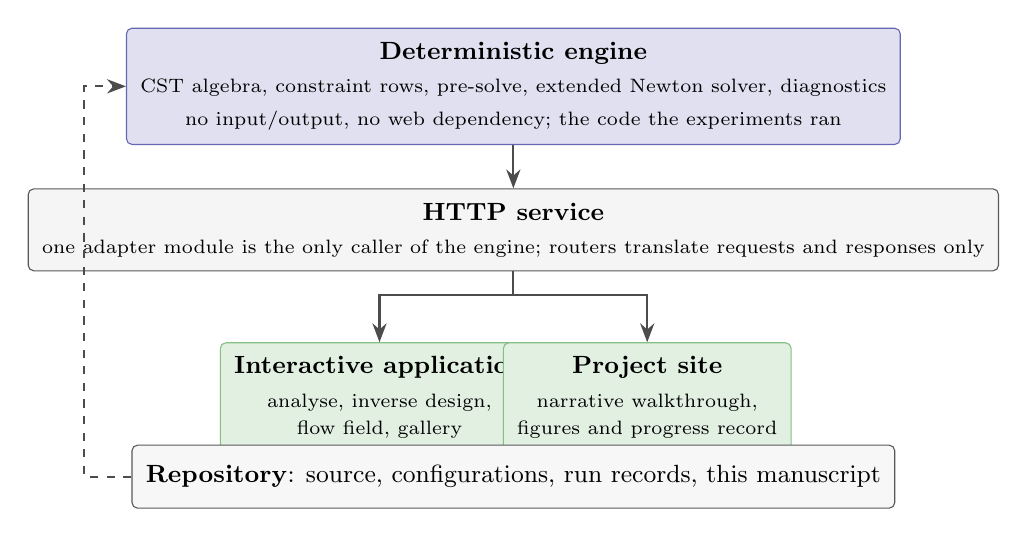
\begin{tikzpicture}[node distance=5.5mm and 12mm]
  \node[fcstart, minimum width=68mm] (engine)
    {\textbf{Deterministic engine}\\[1pt]
     \scriptsize CST algebra, constraint rows, pre-solve, extended Newton
     solver, diagnostics\\[1pt]
     \scriptsize no input/output, no web dependency; the code the experiments ran};
  \node[fcbox, below=of engine, minimum width=68mm] (api)
    {\textbf{HTTP service}\\[1pt]
     \scriptsize one adapter module is the only caller of the engine;
     routers translate requests and responses only};
  \node[fcout, below=9mm of api, xshift=-17mm, minimum width=32mm] (web)
    {\textbf{Interactive application}\\[1pt]
     \scriptsize analyse, inverse design,\\[-1pt]
     \scriptsize flow field, gallery};
  \node[fcout, below=9mm of api, xshift=17mm, minimum width=32mm] (site)
    {\textbf{Project site}\\[1pt]
     \scriptsize narrative walkthrough,\\[-1pt]
     \scriptsize figures and progress record};
  \node[fcbox, below=22mm of api, minimum width=68mm, fill=black!3] (repo)
    {\textbf{Repository}: source, configurations, run records, this manuscript};
  \draw[fcarrow] (engine) -- (api);
  \draw[fcarrow] (api.south) -- ++(0,-3mm) -| (web.north);
  \draw[fcarrow] (api.south) -- ++(0,-3mm) -| (site.north);
  \draw[fcarrow, dashed] (repo.west) -- ++(-6mm,0) |- (engine.west);
\end{tikzpicture}
\caption{The released artifacts. The engine is the code the experiments ran;
everything above it is an adapter, and nothing above it can change a result.}
\label{fig:artifact-stack}
\end{figure}

\subsection{The interactive application}

A deployed web application~\citep{cinsapp} exposes the method to a reader who
does not want to install anything. It is a Python service wrapping the engine,
with a browser front end, and it offers the four views shown in
Figure~\ref{fig:app-views}. \emph{Analyse} runs a direct
coupled solve for a section chosen from the same 123-file coordinate corpus
the panel of Section~\ref{sec:h1-uiuc-panel} was drawn from, or from a NACA
code, and reports the pressure distribution, the boundary-layer state, and the
CST-derived engineering parameters, being leading-edge radius, trailing-edge
wedge half-angles, maximum thickness and camber with their locations, and
inscribed area, all evaluated in closed form from the coefficients by the same
Beta-function machinery as Eq.~\eqref{eq:area-beta} rather than by quadrature.
\emph{Inverse design} runs the monolithic solve itself, iteration by
iteration, in either of two modes: a self-consistency solve against a target
generated from a section's own fit, which is the experiment of
Section~\ref{sec:falsifiable}, or a solve against a target the user supplies
as a pressure or edge-velocity curve. \emph{Flow field} renders the inviscid
velocity and pressure field around the section. \emph{Gallery} replays the
archived results and figures this manuscript reports.

Two behaviours of the user-supplied-target mode are worth recording here,
because they are the product-side evidence for
Section~\ref{sec:le-identifiability}'s finding. First, the realisability
verdict is always reported and never blocks: a target outside the
CST-representable manifold produces a warning carrying the
inviscid-consistent metric of Section~\ref{sec:presolve}, not an error, which
is the reporting rule of that section made into interface behaviour. Second,
the same station-restriction rule the panel runs use is applied here, and it
was in fact found here first. On a user-defined viscous target the
unrestricted candidate set converged in 14 iterations to a surface $0.86$
millichords from the target, while restricting candidates to stations aft of
the prescribed nose converged in 8 to $0.017$ millichords, a fiftyfold
improvement in recovered shape at an almost unchanged residual. Recovery on
such a target is reported and asserted on the \emph{shape} rather than on the
coefficients, because the CST basis is ill-conditioned in $A$
(Section~\ref{sec:nsweep}) and coefficient vectors differing by
$1.8\x10^{-2}$ describe surfaces differing by less than half a millichord;
against a target that only ever constrained pressure, the coefficient norm is
not a meaningful accuracy statement.

\begin{figure}[htbp]
\centering

\includegraphics[width=\textwidth]{paper/fig_app_views.png}
\caption{The four views of the deployed application, captured from the running
service: (a)~analyse; (b)~inverse design; (c)~flow field; (d)~gallery.}
\label{fig:app-views}
\end{figure}

Figure~\ref{fig:app-views} is worth reading against the formulation rather than
as a product tour. Panel~(a) shows the engineering parameters of
Eq.~\eqref{eq:endpoint} and Eq.~\eqref{eq:area-beta} evaluated on a solved
section, which is the closed-form geometric-functional machinery of
Section~\ref{sec:constraints} exposed directly rather than inferred from
coordinates. Panel~(b) is the inverse problem as the user states it, a baseline
geometry, a target pressure curve, and an optional constraint row, which is
precisely the three-block decomposition of Eq.~\eqref{eq:jacobian-blocks}
presented as a form; the constraint panel is also where the target-consistent
right-hand-side rule of Appendix~\ref{app:area} is enforced, since a
leading-edge row added there is built from the pre-solved guess rather than
from an idealised value. Panel~(c) shows the inviscid field beside the coupled
boundary layer, which is the split Section~\ref{sec:transition} depends on.
Panel~(d) replays archived runs, so the evidence behind
Section~\ref{sec:results} can be inspected without a solve.

Two limitations of the deployment are stated so that a reader who tries it is
not misled. The service runs one inverse solve at a time by construction,
because the forced-transition closure of Section~\ref{sec:transition} replaces
module-level functions in the vendored solver and is therefore process-global
rather than instance-scoped; a second submission waits rather than running
concurrently. And the rendered flow field is inviscid, since the
displacement-thickness source contribution is not yet added to it, while the
boundary-layer quantities displayed beside it come from the fully coupled
solve.

\subsection{The project site and the repository}

A project site~\citep{cinssite} presents the method as a narrative walkthrough, from the
problem statement through the linearity argument, the square system, the
falsifiable test, the identifiability finding and the conditioning cliff, using
the same figures as this manuscript. It exists because the argument of
Section~\ref{sec:cst-linearity} is visual before it is algebraic, and a reader
deciding whether to spend time on the formulation is better served by the
figures than by the equations.

The repository carries the engine, the configuration files that define every
run reported here, the archived run records those runs produced, the figure
scripts, the test suite, and the source of this manuscript.
Appendix~\ref{app:repro} states the reproduction procedure and the software
environment; Appendix~\ref{app:prov} maps each figure and table in this
manuscript to the record it was produced from. The vendored flow solver is
included unmodified under its own licence and is never edited; all access to
it passes through a single adapter module, which is what made the
forced-transition closure of Section~\ref{sec:transition} implementable
without a fork.


% =====================================================================
\section{Discussion}
\label{sec:discussion}
\subsection{A common structure across the four mitigations}
\label{sec:mitigations}

The mitigations adopted in this paper are not independent engineering fixes.
Each was arrived at separately, from direct numerical evidence, a stalled
residual, a spiked row norm, a badly conditioned submap, and the common
structure was recognised only afterwards. Recording it is worth a paragraph,
because it suggests where to look first when the architecture is carried into
a solver where the specific failures differ.

Three of the four resolve a tension by separating the two things in conflict
rather than by compromising between them. The transition closure of
Section~\ref{sec:transition} separates them in \emph{time}: the conflict is
between a smooth, Newton-tractable residual and an accurate transition model,
and it is resolved by phase, forcing transition during the inverse iterations
and releasing it afterwards, with a verification solve confirming that nothing
was lost. Nothing is traded away in the end state; the kink is removed exactly
when Newton needs it removed. The prescribed leading edge separates them in
\emph{space}: the conflict is between design freedom, invert everywhere, and
row conditioning, since the residual rows near the nose blow up, and it is
resolved by prescribing the first few percent of chord geometrically and
inverting only aft of it. That does cost design freedom, and
Section~\ref{sec:limitations} records the cost rather than explaining it away.
The station-restriction rule of Section~\ref{sec:le-identifiability} separates
them along the same axis, one level down: having removed a region from the
design space, the sampling must be removed from it too.

The remaining two resolve their tension by improving the quality of what is
already there rather than by adding machinery. For the basis-conditioning
mode, the obvious fix, Tikhonov regularisation, turns a determined solve back
into a least-squares problem, which is the optimisation this architecture
exists to avoid; the discipline adopted instead is to keep the basis order
inside its well-conditioned regime, or to orthogonalise the basis, rather than
regularise a badly-conditioned one. For station selection, adding more target
equations would over-determine the square system, and accepting whatever
stations are convenient is what produced the wrong root of
Section~\ref{sec:ablations}; the resolution reuses an operator the pre-solve
had already built to choose which $M$ rows are maximally informative. Both are
instances of the same instinct: when a determined formulation is the point,
the fix must not add degrees of freedom.

\subsection{Threats to validity}
\label{sec:validity}

The most important limitation of this study is structural and is stated first
because it conditions how every accuracy number in
Section~\ref{sec:results} should be read. No result reported here recovers a
geometry from a target that was produced independently of the method. In every
case, the self-consistency test, the ablation matrix and both panels, the
target pressure distribution is generated by the same solver, at the same
paneling, from a coefficient vector that is exactly representable in the same
CST basis at the same order. Recovery errors at the $10^{-11}$ level are
therefore measurements of \emph{identifiability and conditioning}, showing
that the sampled square system has the generating design as its unique
reachable root and that the Newton iteration finds it, and not measurements of
accuracy against independent data. This is deliberate: a self-generated target
is the only construction under which a failure isolates cleanly to one of the
Table~\ref{tab:fm} failure modes rather than to target infeasibility, which is
what makes the test falsifiable in the first place. But it means the reported
precision does not transfer to a target drawn from experiment, from a finer
discretisation, or from a different solver. The nearest thing to evidence outside this regime is the
user-supplied-target path described in Section~\ref{sec:artifacts}, which
recovers shape to a fraction of a millichord while leaving coefficients to
differ at the $10^{-2}$ level. Even that solve was run against a
self-generated target, and its coefficient gap is attributable to the
inviscid pre-solve meeting a viscous target and to the basis conditioning of
Section~\ref{sec:nsweep} rather than to target independence, so it bounds
nothing. A genuinely independent target has not been attempted, and doing so
is the first item of future work.

Two further gaps in the evidence follow from the same source. The
realisability guard of Section~\ref{sec:presolve} is never exercised on an
unrealisable target: measured realisability on the reference configuration is
$3.90\x10^{-4}$ against a threshold of $0.05$, because a self-generated target
is realisable by construction, so the guard's discriminating power is asserted
rather than demonstrated. And there is no robustness study: real inverse
targets are noisy, over- or under-specified, and nothing here tests target
perturbation or a target that is only nearly realisable. Given that the
identifiability mechanism of Section~\ref{sec:ablations} is a statement about
how much information the sampled rows carry, a sweep of recovery error against
target-noise amplitude is the single cheapest experiment that would sharpen
this paper's central finding, and it has not been run.

The discretisation is also fixed throughout. Every result uses the same panel
count, and for a method whose target rows attach to surface stations and whose
flow-block Jacobian is a finite difference over geometry, sensitivity to panel
count is a first-order question that this study does not answer.

\subsection{Scope limits}
\label{sec:limitations}

The ablation evidence is single-airfoil and single-run. The order sweep, the
station-selection comparison, the remaining single-factor ablations of
Section~\ref{sec:other-ablations} and the cost comparison of
Section~\ref{sec:cost} are all on NACA 2412 at a fixed seed, one run per
configuration, with no confidence interval reported for any of them. That caveat does not extend to the recovery claim itself, which was
upgraded to panel-level evidence across both the 20-section NACA panel and the
117-section UIUC panel (Sections~\ref{sec:h1-panel}
and~\ref{sec:h1-uiuc-panel}); but the ablation-level findings remain
single-airfoil and are not extended to either panel here.

The panel evidence carries a selection effect, quantified in
Section~\ref{sec:h1-uiuc-panel}. Twenty-nine percent of the UIUC panel is
excluded, overwhelmingly because the host analysis solver cannot converge a
target for the section at all, and the excluded sections are systematically
thinner than the converged ones. The exclusion arises before any inverse
problem is posed and is therefore a property of the host solver rather than of
the formulation, but the accuracy claim is conditioned on it. Three further
sections fail the host solver's wake-direction assertion for a cause unrelated
to the sharp-trailing-edge case that an earlier correction addressed; their
trailing-edge gap is already above the minimum, and this remains an open item.

The flow regime is narrow. All results are incompressible: the configuration
sets free-stream Mach number to zero, so the solver's Kármán--Tsien
compressibility correction, which would in any case be valid only below the
critical Mach number, is never exercised. Compressible and transonic behaviour
is untested, as is anything cascade-specific, since there is no periodicity,
no pitch or stagger, and no streamtube contraction. All runs share a single
operating condition, one Reynolds number and one incidence, so no claim here
generalises across flow regimes. The hypothesis under test is a claim about
solver \emph{architecture} rather than about turbine aerodynamics, and is
answered as well on an isolated airfoil as on a cascade; but the regimes the
architecture was ultimately built for are genuinely untested.

Two limits internal to the formulation were flagged in
Section~\ref{sec:contribution} and are repeated here because they bound the
contribution rather than the evidence. The constraint rows, which are half of
the novelty claim, are implemented and unit-tested but not exercised by any
measured result, so wherever an exact analytic constraint-row Jacobian is
offered as an advantage over the nested baseline, it is an advantage of the
formulation and not one this study has measured, in a comparison where neither
side carried an active constraint. And the flow-block Jacobian is obtained by
finite differences rather than from the exact constant geometric sensitivity,
because the host solver exposes no complete geometric sensitivity of its own
residual; the exact sensitivity is used where it can be, in the constraint
rows and the pre-solve, and Section~\ref{sec:h3} measures what the
finite-difference substitute costs in convergence rate.

Finally, the novelty claim itself rests on a negative result established by
open literature search rather than by an exhaustive search of the aerospace
society digital collections. No published work is known that couples a
Newton-coupled inverse solver directly to CST coefficients as Newton unknowns,
as opposed to CST as a post-hoc smoother, but that is a statement about what
was found rather than about what exists.

\subsection{Why the pre-registered cost threshold was missed}
\label{sec:outdated-baseline}

The pre-registered hundredfold claim is not simply missed by the measured
$3.1$ to $8.1\x$ in counted solves, or by the $3.4\x$ in wall-clock time. The
two fair-paired controls of Section~\ref{sec:cost} give a plausible account of
\emph{why} it lands where it does. A Levenberg--Marquardt solve with all three
tolerances at $10^{-8}$ and per-variable scaling taken from the initial guess,
over the same 16 well-conditioned free coefficients, is a genuinely strong
comparator. It converges the cold-start case in six outer iterations, which is
nothing like the surrogate-in-the-loop nested-optimisation baselines that a
hundredfold figure typically describes in the older aerodynamic
shape-optimisation literature the original framing drew on. The pre-registered
threshold plausibly encodes an outdated class of nested baseline. Measuring
against a strong modern gradient-based one and reporting the resulting ratio
directly, in three currencies rather than the most favourable one, is a more
informative comparison than either confirming or missing the original number.


% =====================================================================
\section{Conclusions}
\label{sec:conclusions}
Appending CST coefficients as unknowns to a coupled viscous/inviscid Newton
solver, with geometric design constraints expressed as the linear rows CST's
own linearity makes available, converts constrained inverse airfoil design
from a search over an objective function into a single square, determined
root-find. The falsifiable self-consistency test of
Section~\ref{sec:falsifiable} passes with a wide margin on every accuracy and
iteration-count criterion, including a release-and-verify check the original
protocol had not required, though its convergence rate is fast superlinear
rather than quadratic (Section~\ref{sec:h3}).
The ablation matrix of Section~\ref{sec:results} confirms the architecture's
viability across three NACA sections and Bernstein orders up to a conditioning
cliff at $n=12$, and the two pre-registered panels extend the recovery claim
to 18 of 18 eligible NACA sections and 83 of 83 converged UIUC sections,
subject to the selection effect Section~\ref{sec:h1-uiuc-panel} quantifies.

Two of the study's results correct the hypothesis stated in
Section~\ref{sec:headline}. The cost
advantage over a competently-tuned nested baseline is $3.1$ to $8.1\x$ in
counted flow solves and $3.4$ to $3.5\x$ in wall-clock time, not the two to three
orders of magnitude assumed a priori. And the convergence behaviour is fast
superlinear rather than guaranteed quadratic, limited by the
finite-difference flow-block Jacobian and, under interpolated station
addressing, by a neglected term in the target rows. Against those corrections
stands a methodological contribution the original hypothesis did not
anticipate: QR-pivoted station selection as the identifiability guard for
square inverse systems, without which the same solver converges cleanly to a
wrong root while reporting success. The paper's central results are therefore
a falsified numeric hypothesis and a strengthened, unanticipated qualitative
one.

\paragraph{Future work.} The single most valuable next experiment is the one
Section~\ref{sec:validity} names: recovering a geometry from a target this
method did not generate, whether from a finer discretisation, a perturbed
distribution, or a published pressure distribution, together with a sweep of
recovery error against target noise. Until that is run, the precision reported
here is a statement about identifiability rather than about accuracy.

Beyond it, two extensions are pre-planned and neither is yet built. Cascade
periodicity substitutes a periodic kernel for the isolated-airfoil
panel-influence kernel, replacing $\ln(z-z_0)$ with $\ln[\sin(\pi(z-z_0)/s)]$
for pitch $s$, which reduces to the isolated-airfoil kernel as $s\to\infty$
and therefore comes with a free regression test; it would be validated against
exact cascade solutions before any turbine-cascade inverse-design claim is
made. Carrying the architecture into MISES itself uses that solver's modal
inverse mode. Because CST's perturbation modes are identical to its own basis
functions, a direct consequence of the linearity of
Section~\ref{sec:cst-linearity}, this requires writing $C(\psi)S_i(\psi)$ into
the solver's mode-file format with no modification to its source, and would
demonstrate the hypothesis in a transonic, viscous, real-cascade solver at
near-zero implementation cost if that route succeeds.

The gap between what this paper can currently claim and what was originally
pre-registered is threefold. The single-run ablation evidence has not been
extended to panel level. Three UIUC sections still fail the host solver's
wake-direction assertion for a cause unrelated to sharp trailing edges. And
the constraint rows, which are half of the formulation's novelty claim, remain
implemented and tested but unexercised by any measured result.


% =====================================================================
\section*{Data and code availability}
All source, configurations, run manifests and figure-generation scripts are
available at \url{https://github.com/SharathSPhD/CINS}, together with the
deployed application and the project site described in
Section~\ref{sec:artifacts}. Every figure in this manuscript is regenerable
from the archived configuration and run record that Appendix~\ref{app:prov}
names for it, under the procedure of Appendix~\ref{app:repro}. The flow
solver is \texttt{mfoil}, used unmodified as a vendored dependency.

\section*{Acknowledgements}
The author thanks Krzysztof Fidkowski for releasing \texttt{mfoil} under the
MIT licence, which made a Newton-coupled viscous solver with an accessible
global system available for this work, and Michael Selig and the University
of Illinois at Urbana--Champaign for maintaining the public airfoil
coordinate database from which the evaluation panel of
Section~\ref{sec:h1-uiuc-panel} was drawn.

% =====================================================================
\appendix
% Renders appendix headings as "Appendix A. Title" while leaving \ref
% returning the bare letter, so "Appendix~\ref{app:area}" reads "Appendix A".
\makeatletter
\renewcommand{\@seccntformat}[1]{Appendix~\csname the#1\endcsname.\quad}
\makeatother
\section{Beta-function area-row derivation}
\label{app:area}

\S\ref{sec:constraints} states the inscribed-area constraint row as a
closed-form Beta function without deriving it; this appendix supplies the
algebra (source: \dossierref{\S3.4}).
The per-surface area under Eq.~\eqref{eq:surfaces} is
\begin{equation}
  \mathcal{A}_{\text{surf}} = \int_0^1 \zeta(\psi)\,d\psi
  = \int_0^1 \Big[C(\psi)\sum_i A_i S_i(\psi) + \psi\,\zeta_T\Big]\,d\psi
  = \sum_i A_i \int_0^1 C(\psi)S_i(\psi)\,d\psi + \frac{\zeta_T}{2},
\end{equation}
using linearity of the integral (itself a consequence of
Eq.~\eqref{eq:surfaces}'s linearity in $A$, \S\ref{sec:cst-linearity}) and
$\int_0^1\psi\,d\psi=1/2$ for the trailing-edge term. The remaining integral,
per basis function $S_i(\psi)=K_i\psi^i(1-\psi)^{n-i}$ with
$K_i=\binom{n}{i}$ and $C(\psi)=\psi^{N_1}(1-\psi)^{N_2}$, is
\begin{align}
  \int_0^1 C(\psi)S_i(\psi)\,d\psi
    &= K_i \int_0^1 \psi^{N_1}(1-\psi)^{N_2}\,\psi^i(1-\psi)^{n-i}\,d\psi \\
    &= K_i \int_0^1 \psi^{\,i+N_1}(1-\psi)^{\,n-i+N_2}\,d\psi.
\end{align}
The Euler integral of the first kind is, by definition,
$B(p,q) = \int_0^1 t^{p-1}(1-t)^{q-1}\,dt$ for $\Re(p),\Re(q)>0$. Matching
exponents, $p-1 = i+N_1 \Rightarrow p = i+N_1+1$ and
$q-1 = n-i+N_2 \Rightarrow q = n-i+N_2+1$, giving exactly
Eq.~\eqref{eq:area-beta}:
\begin{equation}
  \int_0^1 C(\psi)S_i(\psi)\,d\psi = K_i\,B(i+N_1+1,\;n-i+N_2+1).
\end{equation}
For the default round-nose/sharp-tail class ($N_1=0.5$, $N_2=1.0$), this is
$K_i\,B(i+1.5,\,n-i+2)$, always well-defined since $i+1.5>0$ and
$n-i+2>0$ for every $i\in\{0,\dots,n\}$, so no term in the sum is singular
despite the class function's own $\sqrt\psi$ non-analyticity at $\psi=0$
(\S\ref{sec:constraints}'s point that the LE singularity affects flow-
residual \emph{rows}, not CST's own geometric \emph{functionals}, which stay
perfectly regular). Stacking one such row per coefficient
gives the full area constraint row $g$ in $g\cdot A = b$, with $b$ the
target inscribed area (or, for the T7/T8 self-consistency protocol, the
area of the CST fit itself, per the target-consistent-RHS discipline
$b=g\cdot A^\ast$ established at T4: the constraint right-hand side must
always be built from what the reference geometry \emph{actually has}, never
from an idealised or rounded value, or the constraint row itself introduces a
spurious residual floor no Newton iteration can remove).

\section{DOF accounting worked example (T7 configuration)}
\label{app:dof}

Eq.~\eqref{eq:dof} ($M+K=n_{A,\text{free}}+n_\alpha$) is an assertion, not a
derived quantity (\S\ref{sec:newton-system}); this appendix works it for the
T7 winning configuration and states the general rule it specialises.

\paragraph{The T7 case.} $n=8$ per side $\Rightarrow$ 9 coefficients per
surface, 18 total ($A_{u,0..8}$, $A_{l,0..8}$). \texttt{le\_treatment=
prescribed} removes 2 of these from the free set: $A_{u,0}$ and $A_{l,0}$
are geometrically fixed to the reference fit's own values, not Newton
unknowns (\S\ref{sec:falsifiable}), leaving $n_{A,\text{free}}=16$. Because
$A_{u,0}/A_{l,0}$ are prescribed directly
rather than tied by an equality row, no separate shared-LE constraint row is
needed for this configuration: $K=0$. $\alpha$ is fixed for the
self-consistency protocol (removing the camber--$\alpha$ null direction,
\S\ref{sec:ablations}): $n_\alpha=0$. Eq.~\eqref{eq:dof} therefore requires
$M = 16 + 0 - 0 = 16$ target-station equations, exactly the QR-pivoted
station count reported throughout \S\ref{sec:falsifiable}--\S\ref{sec:ablations}
(\pth{experiments/results/t7_naca2412/diagnostics.json}, \texttt{static.
dof\_accounting}: \texttt{n\_A\_free=16, M=16, K=0}).

\paragraph{The general rule.} Restating Eq.~\eqref{eq:dof} in full generality:
for $n$ Bernstein coefficients per surface (2 surfaces, so $2(n+1)$ raw
coefficients), $c_{LE}\in\{0,1\}$ constraint rows tying the leading-edge
coefficients (shared-LE row, used only when \texttt{le\_treatment=none} or
\texttt{lem}, not when \texttt{prescribed} pins the coefficients directly),
$p_{LE}\in\{0,2\}$ coefficients removed by prescription (2 when
\texttt{le\_treatment=prescribed}, else 0), and any additional geometric
constraint rows $K_{\text{extra}}$ (TE thickness, inscribed area, curvature,
\S\ref{sec:constraints}):
\begin{equation}
  n_{A,\text{free}} = 2(n+1) - p_{LE}, \qquad K = c_{LE} + K_{\text{extra}},
  \qquad M = n_{A,\text{free}} + n_\alpha - K.
\end{equation}
This is the Stage-1 (isolated-airfoil) specialisation of the dossier's
original rigid-body bookkeeping
(\S\ref{sec:newton-system}'s $\mathrm{DOF}=2(n+1)-1_{\text{shared LE}}-
1_{\text{TE fixed}}+3_{\text{scale/rotate/translate}}+1_{\text{stagger or
}\alpha}$): the three rigid overall modes are not exposed as free Newton
unknowns in this implementation (chord, position and rotation are fixed by
convention, not solved for), so they contribute neither to
$n_{A,\text{free}}$ nor to $M$, and Eq.~\eqref{eq:dof} is the resulting
simpler, directly-assertable statement. The rule's lineage is Lighthill's
own well-posedness bookkeeping~\citep{lighthill1945new}: a conformal-mapping
inverse solve is well-posed only when the number of free shape parameters
exactly matches the number of independent closure conditions (contour
closure, LE radius, circulation) the target and geometry family jointly
admit. Eq.~\eqref{eq:dof} is that same counting argument, discretised for
a finite-dimensional CST basis and asserted programmatically rather than
checked by hand.

\section{The onset-closure Jacobian rows}
\label{app:onset}

\S\ref{sec:transition} describes \texttt{\_residual\_transition\_forced}
(ADR-0003) narratively; this appendix states its Jacobian-row structure
explicitly, since it is the one residual block in this paper's extended
system that is not simply reused unchanged from mfoil
(\S\ref{sec:newton-system}). At a forced-transition onset station with
endpoint states $U_1$ (upstream, still formally laminar-indexed) and $U_2$
(downstream, freshly turbulent), the vendor three-row station residual is
$R=[R_{\text{mom}},\,R_{\text{shape}},\,R_{\text{lag}}]$
(\texttt{mfoil.py}, \texttt{residual\_station}). Rows 0--1
(momentum, shape parameter) are vendor's own ordinary turbulent closure
evaluated directly across $[x_1,x_2]$: an unchanged code path, so their
$U$- and $x$-Jacobian blocks are exactly mfoil's own
$\partial R_{\text{mom},\text{shape}}/\partial U_{1,2}$,
$\partial R_{\text{mom},\text{shape}}/\partial x$, reused verbatim. Row 2
(shear-lag) is replaced with the onset condition
$U_2[2] - c_{ttr}(U_2) = 0$, where $c_{ttr}$ is the same transition-
correlation root-shear-stress function (\texttt{get\_cttr}) vendor's own
\texttt{update\_transition} uses to initialise a newly-turbulent node.
Because $c_{ttr}$ is a function of $U_2$ (specifically $\theta,H_k,Re_\theta,
u_e$ at the downstream node) only, its Jacobian row has the structure
\begin{equation}
  R_U[2,\,0{:}4] = 0 \quad(\text{no } U_1 \text{ dependence}), \qquad
  R_U[2,\,4{:}8] = e_{sa} - \left.\frac{\partial c_{ttr}}{\partial U_2}\right|_{U_2},
  \qquad R_x[2,\,:] = 0,
\end{equation}
where $e_{sa}=[0,0,1,0]$ selects the shear-lag component of $U_2$ and
$\partial c_{ttr}/\partial U_2$ is \texttt{get\_cttr}'s own analytic
derivative block (\texttt{cttr\_U}), already computed by vendor code for the
identical purpose inside \texttt{update\_transition}: reused, not
re-derived. The row's independence from $U_1$ and from $x$ is not an
approximation: it follows structurally from $c_{ttr}$'s own functional
form, which was verified by direct inspection of \texttt{get\_cttr}
(ADR-0003, ``Modeling choice''), and it is what makes this replacement
row well-defined at a station where the natural (unforced) closure's
internal $x_t$-solve has no solution (\S\ref{sec:transition}).

\section{Reproducibility statement}
\label{app:repro}

\begin{itemize}
\item \textbf{Repository.} \url{https://github.com/SharathSPhD/CINS.git}
  (branch \texttt{main} at every gate closure, per this project's workflow
  discipline). \pth{vendor/mfoil/mfoil.py}~\citep{fidkowski2022coupled}
  is vendored unmodified (MIT licence) and is never edited; all solver
  access is through \pth{src/cins/solver/mfoil_adapter.py}.
\item \textbf{Manifest scheme.} Every experiment run in this paper writes
  an immutable manifest under \pth{experiments/results/} recording the
  git SHA, a hash of the fully-resolved \pth{configs/*.yaml} used, the
  random seed (\texttt{experiment.seed}, \texttt{42} throughout), and
  enough metadata to regenerate the run byte-for-byte
  (\citep{cinsrepo} condition~4). No number in this paper is
  hand-edited; every table cell traces to a \texttt{result.json} or
  \texttt{diagnostics.json} artifact under \pth{experiments/results/},
  cited inline by path throughout \S\ref{sec:falsifiable}--
  \S\ref{sec:results}.
\item \textbf{One-command regeneration.} T8 ablation-matrix figures (D-6
  overlay, $n$-sweep, flow-solve bar chart, station-selection comparison):
  \texttt{.venv/bin/python -m cins.benchmarks.figures}. This paper's new
  geometry/Cp/flow-solution/H1-gallery figures
  (\S\ref{sec:falsifiable}, \S\ref{sec:h1-panel}): \texttt{.venv/bin/python
  -m cins.benchmarks.paper\_figures}. Both re-run the underlying
  monolithic solves fresh rather than reading cached scalars, since neither
  \texttt{t7\_naca2412/diagnostics.json} nor any \texttt{t8/*/result.json}
  stores the CST coefficient vectors or field distributions themselves
  (only scalar summaries; verified directly against the on-disk schema
  before writing \texttt{paper\_figures.py}, not assumed). Individual T7/T8
  cells: \texttt{.venv/bin/python experiments/run\_t7.py} and
  \texttt{.venv/bin/python -m cins.benchmarks.runner} respectively. Tests:
  \texttt{python -m pytest tests/ -q}.
\item \textbf{Gate-closure evidence.} \citep{cinsrepo},
  \texttt{T3-closure.md}, \texttt{T4-T7-closure.md} record the six-condition
  gate-closure contract (\citep{cinsrepo}) for each corresponding
  task, including adversarial-review findings and their resolution;
  \citep{cinsrepo} through \texttt{ADR-0004} record the four
  binding architectural decisions this paper's Formulation section depends
  on (scipy shim, vendor NACA5 shim, forced-transition shim, realisability
  semantics).
\end{itemize}

\bibliographystyle{plainnat}
\bibliography{p1_refs}


% =====================================================================
\bibliographystyle{plainnat}
\bibliography{p1_refs}

\end{document}
